% vim:ft=tex
\documentclass[a4paper,11pt]{scrartcl}
\usepackage{tohojo-xe}
%\selectlanguage{english}
\setcounter{secnumdepth}{3}
\setcounter{tocdepth}{2}
\hypersetup{pdfauthor={Toke Høiland-Jørgensen, Mikkel Hartmann, Dan 
Albrechtsen, Malik Thrane, Troels Christensen, Wence Xiao}, pdftitle={Crowd 
modelling}}

\title{Crowd modelling}
\author{Toke Høiland-Jørgensen, Mikkel Hartmann, Dan Albrechtsen, Malik 
Thrane, Troels Christensen, Wence Xiao}
\date{2010-09-12}
\fancyhead[OR,EL]{\footnotesize Draft: \timestamp}
%\type{}
 
 
\begin{document}

\begin{titlepage}
    \begin{center}
        {\Huge \sffamily \textbf{Crowd modelling\\[2cm]
        }} Picture here %\includegraphics[width=15cm]{figurer/forside}
        \\[2cm]

        {\large Toke Høiland-Jørgensen \\
        Mikkel Hartmann\\
        Dan Albrechtsen\\
        Malik Thrane\\
        Troels Christensen\\
        Wence Xiao\\
        [0.5cm] }

        {\small \textbf{\textsf{Advisor}}\\
        Viggo Andreasen}
        \vfill
        \textsf{Modelling project, fall 2010\\
        Mathematics RUC}
	\end{center}

    \clearpage
%    % vim:ft=tex

\begin{abstract}
    \section*{Abstract}
    \small
    We look at social force models as a way to model the behaviour of human 
    crowds, in order to evaluate what these types of models can tell us about 
    crowds, which assumptions underlie them and what their strengths and 
    weaknesses are. In order to do this evaluation, we implement a computer 
    simulation of an exemplary social force model.

    In order to create this simulation, we pick an exemplary model that is 
    described in detail in the article that presents it, and analyse it in 
    detail, filling in details from other articles where necessary. Based on 
    this analysis of the model, we go from the abstract model formulation to a 
    concrete numerical simulation by filling in required details, such as  how 
    to approximate the movement of pedestrians, how to set initial conditions 
    and values, and how to implement the interaction between pedestrians and 
    walls in practice.

    From our results, it is clear that our simulation (with the right 
    parameters) exhibits reasonable pedestrian behaviour upon visual 
    inspection. While we successfully replicate some results from the 
    literature, other effects do not manifest themselves. We discuss several 
    reasons for this discrepancy, including features that are lagging from the 
    model, parameter values, effects of using random numbers to generate the 
    initial conditions and possible errors in our implementation of the model.

    Based on the results of our own simulations and our review of the social 
    force modelling field, we assess social force models and their strengths 
    and weaknesses. We conclude that social force models are not built on any 
    theories for the behaviour of crowds, but are created to replicate a set 
    of observations. As such, any confidence in their predictions must come 
    from a record of producing results fitting observations; and since the 
    field is relatively new, they have not yet reached this state. Social 
    force models do, however, provide a practical way to simulate something 
    that would otherwise be impossible to simulate. As such, they are the best 
    available way to provide e.g. guidance when designing facilities that must 
    accommodate many pedestrians, and given time the accuracy of their 
    predictions will probably increase.
\end{abstract}
\begin{abstract}
    \section*{Resume}
    \small
\end{abstract}

\end{titlepage}

\tableofcontents
\listoffigures

\clearpage

% vim:ft=tex
\section{Introduction}
When a lot of people are gathered in a confined space, it is not immediately 
obvious how they behave when moving around. It is also not obvious how to 
design buildings and other areas where many people gather to allow for optimal 
passage of crowds without jamming and related problems (such as inconvenience 
for pedestrians and even injuries). It is cumbersome, or even dangerous, to 
gather many people together to do experiments, especially if one wishes to 
simulate a panic situation (which cannot necessarily be induced artificially).  
It would thus be useful to be able to model a crowd of pedestrians and their 
movement.

A crowd of many people is a very complex system. One of the approaches to 
handling this complexity is by using a computer simulation of a model derived 
from the behaviour of individual pedestrians, and through the outcome of this 
simulation be able to say something meaningful about the whole system. This 
approach to modelling complex systems is called agent-based modelling and is 
used in many different and diverse subject areas, including molecular biology, 
economics and physics.

Within the field of crowd simulations, there  are various ways of formulating 
such an agent-based model; we have chosen to focus on an approach that models 
pedestrian behaviour using a concept called ``social forces'' 
\cite{social-force}. This type of model describes individual behaviour 
borrowing concepts and notation from physics, by defining  virtual ``forces'' 
representing desired movement as well as the tendency to avoid obstacles, 
other people etc. Through computer simulations this can be used to say 
something about the whole system of moving pedestrians.

Since the original formulation of the social force concept, it has been 
revised several times (e.g.  \cite{helbing00}). For this project we base our 
analysis on the  version presented in \cite{self-org}, as this article goes 
into a reasonable level of detail. We will, however, also include other 
variants where necessary.  Our chosen model, and others like it, describe a 
set of properties of crowd behaviour that has been seen in observations of 
actual crowds as well as replicated in computer simulations.  We think it will 
be interesting to go into detail with this type of model and look into how 
they work and what they can tell us about crowds. This brings us to our 
problem formulation:

\subsection{Problem formulation}
\begin{quote}
    How do social force models work and what do they say about crowds?

    What are the assumptions underlying social force models, and what are 
    their strengths and limitations?
\end{quote}

Our problem is exemplary to mathematical modelling for several reasons. First 
of all, it is an example of applying mathematical theory to a field outside of 
mathematics itself. The field we are working with (crowd simulation) is 
relatively new, but has some established research\footnote{See the overview of 
the field in section~\ref{sec:social-forces}.}. The model itself contains a 
non-trivial application of mathematics and is an example of a type of model 
(agent-based models) used in many cases to study a complex system of 
interacting pedestrians by describing the individual behaviour of the pedestrians and 
using simulations to derive meaningful properties for the whole system. These 
factors combined makes our problem exemplary.
% TODO: References for agent-based models.

\subsection{Target audience}
The target audience of this report is comprised of students of mathematics on 
a level of education similar to our own. This means that we consider 
mathematical concepts and theory that is covered in the bachelor courses at 
the mathematics department at RUC as known subject matter, and will therefore 
not explain these concepts in detail. Concepts that are beyond this are 
explained as necessary. In the description of the simulation program code, 
some familiarity with basic constructs of computer programming is assumed, and 
are thus not explained.

\subsection{Approach to answering the problem formulation}
To answer the problem formulation, it is first necessary to establish the 
concept of social force models in more detail, as well as give an overview 
over the work in the field. This is presented in 
section~\ref{sec:social-forces}, where we also present the model we have chosen 
to focus on, including the results presented in it.

In order to better understand the model, we are going to make our own computer 
simulation of it. To do so, we will first describe the model thoroughly. In 
section~\ref{sec:the-model}, we will go over the different parts and 
parameters of the model, and point out parts that are ambiguous or missing 
from the article presenting the model.  Based on this description, we will 
discuss what is needed to turn the model into a numerical simulation, and how 
we have done so, in section~\ref{sec:model-to-simulation}.

Based on our analysis of the model, we will construct a computer simulation of 
it, modelling cases analogous to those presented in 
section~\ref{sec:social-forces}. Our implementation of the 
simulation is discussed in section~\ref{sec:simulation}, including set up of 
parameters and initial conditions, the structure of our simulation and how we 
obtain results from it.

The actual results of the simulation is addressed in 
section~\ref{sec:results}. Here we present the outcome of our simulation, and 
whether or not we have been able to replicate the results we were aiming for.  
Based on this presentation, we discuss in section~\ref{sec:discussion} 
possible reasons for any discrepancies between our own results and the results 
we are trying to replicate, as well as which alterations of the model would 
be needed to fix them.

Based on our results and the proposed changes to the model, we will assess 
social force models in general in section~\ref{sec:assessment}, giving an 
overview of the strengths and weaknesses of this modelling approach. Finally, 
we will give a summary of our findings and an overview of the whole project in 
section~\ref{sec:conclusion}.

\clearpage
\section{Crowds}
\label{sec:crowds}
In this section, we establish some concepts for discussing the behaviour of 
crowds in general, in order to have a basis on which we can analyse our chosen 
model. We also give an overview of the work that has been done in the field of 
crowd modelling and which approaches there has been to tackling this area, as 
well as background information on the type of model (agent-based) we are 
dealing with. Finally, we outline the cases we want to use in our simulations.

\subsection{Agent-based models and their origin}
The modelling of human behaviour using agent-based models is a 
pretty new field in modelling \cite{helbing00}. In this section, we give an 
overview of the use of agent-based models in other areas.

An agent-based model is a model that describes the behaviour of individuals 
and through simulations derive behaviour of the system being modelled.  
Agent-based models are used in many different fields.  They have their origin 
in physics where the idea of agent-based models dates as far back as 1820. 
Back then Laplace wrote \cite{simintro}:

% TODO: Language cleanup etc.

\begin{quote}
    An intelligent being who, at a given moment, knows all the forces that 
    cause nature to move and the positions of the objects that it is made 
    from, if also it is powerful enough to analyze this data, would have 
    described in the same formula the movements of the largest bodies of the 
    universe and those of the lightest atoms. Although scientific research 
    steadily approaches the abilities of this intelligent being, complete 
    prediction will always remain infinitely far away.
\end{quote}

So the main idea of agent-based models and their application has been thought 
of since long before the usage of computers. But it wasn't until the last half 
of the 20th century that it was actually possible to work with agent models 
because of the numbers of calculations needed to make use of 
them \cite{simintro}.  Since then the application of agent-based models have 
been huge and it is now used in many of different fields. 

One of the most well-known and first established (1957 \cite{MDintro}) 
agent-based model simulations is the molecular dynamics (MD)-simulations 
\cite{MDintro}. The idea of MD-models is simply to describe particles moving 
around by calculating the mechanical forces working on each of the particles.  
These kind of models allow you too see what happens with each particle and from 
that it is possible to calculate well known physical properties like 
temperature, pressure and so on . You can even see when there is a phase 
change from liquid to solid and back again. But also you can use it for much 
more complex behavior. In molecular biology and chemistry you can use 
MD-simulations to calculate the behavior of long-chain molecules \cite{MDbio}.  
In these models you even sometime add some stochastic elements to the models.  
This can be used to get some theoretical idea about how reactions happens and 
alot of other things.

But also in fields that you normally wouldn't connect with physics you see the 
application of microscopic models.
One of the more exotic fields to use microscopic models is in financial 
markets \cite{finans}.  In these kind of simulations you can describe how the 
behavior of individuals affects market dynamics.  It is of course not 
mechanical forces that controls this kind of models, but the idea of looking 
at and calculate the effects of the individual is maintained. 

Microscopic models has also been used on different types of animals like fish 
and with good results.  One of the things that have been simulated is fish 
schools \cite{fish}. In these simulations they try to the describe how a fish 
school moves around by calculating the positions of each fish and the effects 
from its nearest neighbours. In these kind of models people get some realistic  
looking behaviours that looks like what you would see in nature. Because of 
this very wide application of agent based models it seems natural to assume 
that it also could be fitted to use on human behaviour. Especially since it can 
be used on other animals, even though it could be argued that you of course 
would expect animals behavior to be more primitive than that of humans and 
therefore more easy to model.  Since microscopic models is used in a lot of 
different ways they also looks very different. That is because only the main 
idea of looking at the individual repeats throughout all of the models. So even 
though microscopic models is used very widely there is still a lot to of 
calculations and considerations that changes when the field changes and 
therefore it is still non-trivial.

\subsection{Social Force models}
%	There should be an introduction to this section.. were going to compare the 		%
%	differnt ways of simulating crowds.. but wait then it's not only relevant for 		%
%	social force models. This might fit better into the Crowds section if its rewitten	%
%	correctly.																			%

%	Some history about the social force model might serve well as an introduction here	%
In this section we will first give a short presentation on Social Force models and their history,
and then compare the features of Social Force models with the features of other models that describes
the behavior of crowds.
\\

The idea behind social force models is that each individual, pedestrian $\alpha$, in the crowd acts 
on her own from a personal aim or goal and by behavioral reactions to the environment. 
Different forces such as other pedestrians, walls and obstacles are taken into account 
when pedestrian $\alpha$ walks toward her aim or goal, so that she does not walk 
into another pedestrian or wall. The forces influencing $\alpha$'s motion 
of direction are not forces acting on $\alpha$'s body, but has to be seen as a quantity 
that describes the motivation to act. Since $\alpha$ is used to the situations 
she is normally confronted with, her reactions will be rather automatic and 
determined by her experience of which reaction will be that best. Since the reaction 
is rather automatic it is possible to put the rules of pedestrian behavior into an equation 
of motion.\cite{social-force}

\subsubsection{Comparison with other crowd models}
There are other ways to model crowds than social force models such as Rule Based models, 
Cellular Automata models and Hybrid models. Below we will make a short explanation of each of the 
other crowd models, and then compare the features of the models.\\												%

\textbf{Rule Based models}\\
Rule Based models describe the movement of pedestrians through sets of basic rules. Each 
pedestrian apply collision detection and avoidance to prevent collision with other pedestrians. 
However they do not in general apply collision response, and therefore collisions and overlappping 
of the pedestrians may occur under some circumstances. Some models have applied stopping 
rules to prevent these situations.\cite{Comparison}

\textbf{Cellular Autamata models}\\
These models are discrete, deterministic and is made up of cells like the squares in a chessboard.
An artificial intelligence approach is used in Celluar Automata (CA) defined as mathematical idealisation 
of physical systems in which time and space are discrete, and physical quantities take a finite set of 
discrete values. Pedestrian can not collide since the floor is dicretised and the pedestrians can
only move to free adjecent cells.\cite{Comparison}

\textbf{Hybrid models}\\
The Hybrid models has been made from social force models and rule based models. 
The motion of the pedestrians is caried out like the social force models, but is also based 
on the psychological and geometrical rules. It peforms collision detection and response and rules 
are applied depending on the pedestrian's personality and the state of the environment. 
\cite{Comparison}
\\

\subsubsection{Geometrical features of the models}
Each of the different models have some geomatrical features relatively important and 
unimportant according to our simulation.

\textbf{Shaking} Wether pedestrians appear to shake when simulating the model. When 
simulating the social force models the pedestrians seems to shake when cloggings and 
queues arise. This is caused by the modification of each pedestrians postition in each 
timestep. The Hybrid, CA and Rule Based model do not appear to shake while the simulation run.

\textbf{Discrete and Continuous movement} Wether the space and time are discretised. In the CA model the pedestrians move between discritised adjecent
cells in one time step, and therefore have limited direction to go. The other models do not discretise space and therefore allow the pedestrians to move
within continuous space.
 
\textbf{Overlapping} Wether overlapping of the pedestrians is possible. The rule based models and the CA models do have collision detection but not
all have collision responce. The CA models have rules so that a pedestrian can not walk into an occupied cell, but if two pedestrians want to pass each
other they step into the cell diagonal to their own cell, and in their way cross the other pedestrian in the intersection between the four cells.
Newer models of the rule based and CA have made a stopping rule so that overlapping can not accour. The Hybrid and social force models do collision responce
to minize the risk of overlapping. \cite{Comparison}

\begin{figure}
    \centering
    {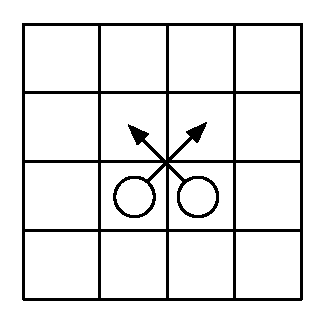
\includegraphics[scale=0.55]{Figures/Overlapping.pdf}} 
    \caption{Sketch of two agents overlapping in a Cellular Autamata model}
    \label{Overlapping}
\end{figure}

\textbf{Pushing} Wether pedestrians can have physical contact. If the pedestrians can have physical contact they will be able to push each other in some
direction. This ability is possible when using the Hybrid and the social force model. When simulating evacuations and chaotic events it has been observed
that people do have physical contact and push each other \cite{self-org}.

\textbf{Communication} Wether the pedestrians can share information about he environment. The HiDAC and som newer rule based models allows the pedestrians
to share information about the environment and to give orders. This feature is not included in social force models and CA. \cite{Comparison}

To illustrate different features of the different models the table below sums up the above mentioned.
\begin{center}
\begin{tabular}{lllll}
 & Social Forces & Rule Based & CA & Hybrid\\
Shaking avoidance     & - & + & + & +\\
Continuous space      & + & + & - & +\\
Overlapping avoidance & + & * & - & +\\
Pushing               & + & - & - & +\\
Communication         & - & * & - & +
\end{tabular}
\end{center}
Here ``+`` indicates that the feature is possible, ``-`` indicates it is not, and ''*'' that the model has been adjusted such that the feature have
become possible. \cite{Comparison}

The features we are interested in and find relevant in our simulation are continuous space, pushing and overlapping avoidance. The continuous space is
relevant for our simulaion to be as realistic as possible since we do not want our pedestrians to have at most nine directions to go each timestep.
The feature of pushing is also important to include since in panic sitiation it has been seen that people push each. This feature will then make our
simulation more realistic.
The overlapping avoidance we find relevant since this enables pedestrians to walk through each other.
\\
Therefore we find that modeling a crowd by using a social force model is most oppropriate in our project. 
%	Finishing off with a conclusion would be neat					%


\subsection{Concepts for describing crowd behaviour}
In order to analyse the behaviour of crowds, we need to establish some 
concepts to describe this behaviour. It is not obvious which concepts  are 
useful when we need to distinguish between the results we get from our 
simulations. In this section we describe which concepts we use to describe the 
behaviour of crowds, and why we have chosen them. This is based on the 
literature of crowd modelling.

One of the reasons for modelling crowds is to discover ways to make crowd 
situations safer for pedestrians, e.g. when evacuating a building in event of 
a fire. One of the main factors in this scenario is the \emph{efficiency} of 
the crowd movement. This is especially important when clearing a room in the 
event of a fire or other disaster: the faster everyone gets out, the lower is 
the chance of someone dying from flames or smoke.

The obvious measure of efficiency is measuring how long it takes to empty a 
given room. This, however, makes the results highly dependent on the specific 
situation we are modelling (i.e. room size, number of people in the room, 
etc.). If we wish to compare results from different cases, we need a measure 
that is less dependent on the room configuration. Such a measure could be the 
\emph{flow rate}, i.e. the number of pedestrians passing a specific point (or 
line) in space per time unit.

% TODO: This section needs to be expanded with more concepts, references to 
% where we get the concepts, as well as a better arguments for why we have 
% chosen exactly these measures.

\subsection{Our case(s)}

Here we will shorty describe our case of the simulation of the model and the environment which the simulation is runned within.
We have chosen to simulate the model in a 10 m. x 10 m. room with one exit, and consisting of 10 pedestrian evenly distribited in the room.
When the simulation starts the pedestrians begin to moves toward the room's exit.
\\
The simple environment has been chosen because we just want to get the simulation up and working, and because we want as cheap a calculation as possible.
Therefore it is not needed to have a complex environment, since this would make the programming more difficult and would use more computation to run
the simulation.
We have only selected 10 pedestrians also due to the fact that we want cheap calculation and the model does not recuire a high density crowd.
\clearpage
\section{The model}
\label{sec:the-model}

\subsection{Explanation of our model}
In this section we will go through the model from the article \cite{self-org} in 
great detail, in the way that we understand the mathematical expressions and also 
see how those expressions represent the reality.\\

\underline{Force analysis:} \\
As the social force model is an agent based model, it focuses on looking at the 
quantities about an individual agent, at last get the motion of the crowd. In order 
to get the equation of motion we always start by analysing the forces acting on the object.\\\\

Here in this model, the agents cannot escape from Newton's three laws of motion, 
which mainly says that when there is a force it results a corresponding acceleration.  
Therefore, it is necessary to look at the forces.  However, our agent is not a ball 
being kicked around, it has a willingness to go to some destine place, and the 
"willingness" to go somewhere is hard to measure, but we know that the way an agent 
implement the will normally is by generating a static frictional force from the ground, 
and that force is here what we called a kind of "social force", which is 
$\vec{f^{0}_{\alpha}}$ in Figure \ref{ForceModel}. 

Some other major forces acting on the agent are the repulsive force from other agents 
namely $ \beta $ - the force called $ \vec{f_{\alpha\beta}} $ in Figure \ref{ForceModel}, 
and repulsive force from an obstacle (a wall for example) - the force called $ \vec{f_{\alpha B}} $ 
in Figure \ref{ForceModel}.  As these two repulsive forces are a kind of normal force, the direction 
should be perpendicular to the surface.

\begin{figure}[hb]
    \centering
    {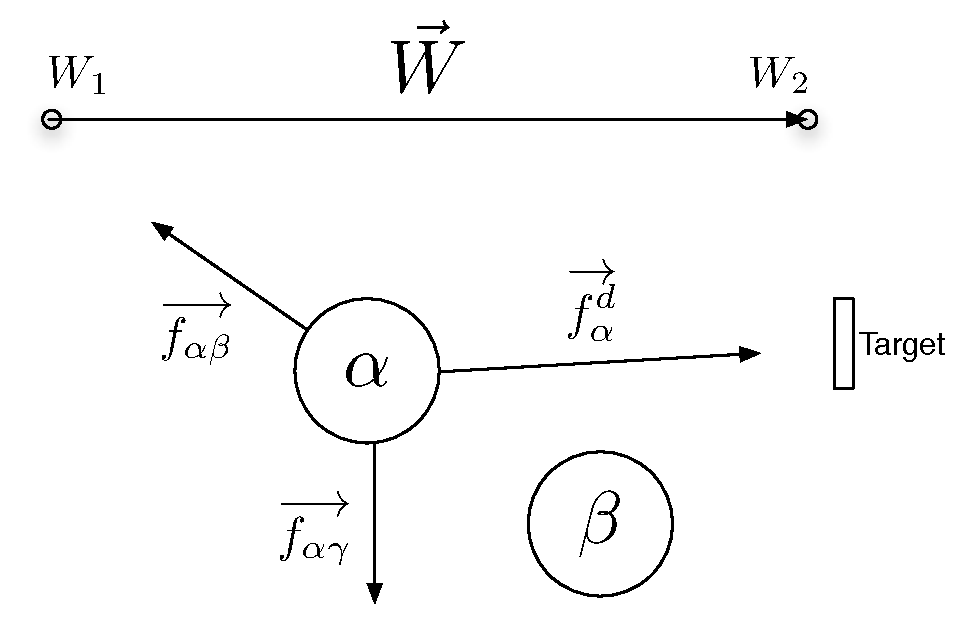
\includegraphics[scale=0.45]{Figures/ForceModel.pdf}} 
    \caption[Notation of forces acting on an agent]{Illustration of the forces acting on an agent $ \alpha $. $ \beta $ is another agent and the grey bar on the top represents a wall. $ \vec{f_{\alpha\beta}} $ is the repulsive force from agent $ \beta $, and $ \vec{f_{\alpha B}} $ is the repulsive force from the wall. $ \vec{f^{0}_{\alpha}} $ is a force that represents agent $ \alpha $'s desire to reach the exit.
    The x and y axes are defined by the Cartesian coordinate system.}
    \label{ForceModel}
\end{figure}

So far in the model it only mentioned the forces on the horizontal level, the gravitational force and normal force from the ground which works vertically are not mentioned at all.  The reason is that in this model they only consider the motion on the horizontal plane.  Since there is no motion vertically, the gravitational force and the normal force from the ground cancel each other.\\\\
\underline{The equation of motion for agent $ \alpha $:}\\

The general approach of the model to get the equation of motion follows the standard way. Summing up the forces acting on $ \alpha $ gives the acceleration, which builds the equation of motion. It comes in steps as the following.\\
First of all, the equation of motion deals with the agent $ \alpha $'s position $ \vec{r_{\alpha}} $, velocity $ \vec{V_{\alpha}} $, and acceleration $ \vec{f_{\alpha}} $. As the agent is not just a mass point, it has a radius $ r_{\alpha} $. The position and velocity vectors and the radius are shown in Figure \ref{NotationOfAgent}.

\begin{figure}[hb]
    \centering
    {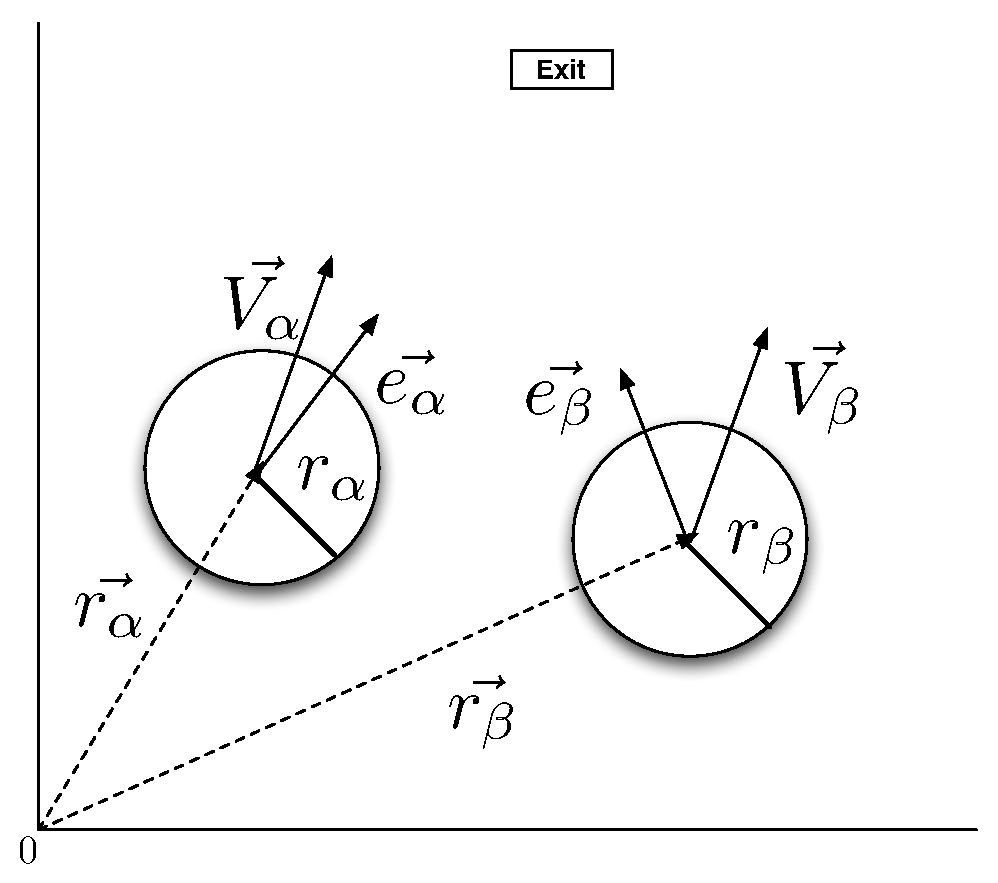
\includegraphics[scale=0.35]{Figures/NotationOfAgent.pdf}} 
    \caption[Notation of an agent]{Illustration of the visual presentation of the mathematical notations for position and velocity. As for agent $ \alpha $,
	    it has position vector $ \vec{r_{\alpha}} $, velocity vector $ \vec{V_{\alpha}} $, $\vec{e_{\alpha}}$ or $\vec{e_{\beta}}$ the normal vector pointing
	    to the exit and  $ r_{\alpha} $ or  $ r_{\beta} $ the radius of its body.
	    The x and y axes are defined by the Cartesian coordinate system.}
    \label{NotationOfAgent}
\end{figure}

The change in position $ \vec{r_{\alpha}} $ per time of 
agent $\alpha$ is actually the velocity $ \vec{V_{\alpha}} $:

\begin{equation}
		\frac{d \vec{r_{\alpha}}}{dt} = \vec{V_{\alpha}} \left( t \right)
\end{equation}

Also known from Newtonian physics, the change of velocity per time is the acceleration of agent $\alpha$, which is the result of a summation of all the forces acting on the agent, namely $\vec{f_{\alpha}} \left( t \right)$:

\begin{equation}
    \frac{d \vec{V_{\alpha}}}{dt} = \vec{f_{\alpha}} \left( t \right) 
\end{equation}

Referring to the part for force analysis, we need to add the driving force, repulsive force from the wall and repulsive force from other agents, also there is attractive force $ \vec{f_{\alpha i}} $ if the agent $ \alpha $ has some relatives or friends in the crowd.

\begin{equation}\label{model}
    \vec{f_{\alpha}} = \vec{f^{0}_{\alpha}} + \vec{f_{\alpha B}} +
    \sum_{\beta \neq \alpha} \vec{f_{\alpha \beta}} +  
    \sum_{i} \vec{f_{\alpha i}} 
\end{equation}

Naturally the work next is to show explicit expression for each force, and we will go through them one at a time explaining their mathematical structure and their role in the model.\\

\subsubsection{The driving force} %gotta figure out a better name for this part
The first term on the right hand side of equation \eqref{model} describes the implement of agent $ \alpha $'s "willingness" to reach the exit. In this model it is a velocity dependent force 
and is given by:

\begin{equation}\label{relaxtime}
	\vec{f^{0}_{\alpha}}\left( \vec{V_{\alpha}} \right) =
    \frac{1}{\tau}
    \left( V_{\alpha}^{0} \vec{e_{\alpha}} - \vec{V_{\alpha}} \right)
\end{equation}
where $V_{\alpha}^{0}$ is the desired speed, $ \vec{e_{\alpha}} $ is the normal vector pointing to the exit, $\vec{V_{\alpha}}$ is the actual velocity of the agent, and $\tau$ is the relaxation time. \\

From Equation \ref{relaxtime} we get the ideas that:
\begin{itemize}
\item About the notation, any quantity with a "$ ^{0} $ " on the upper right corner is a "desired" quantity.
\item Although $ \vec{f^{0}_{\alpha}} $ is a kind of desired force, it actually exists, because it appears in Equation \ref{model} for calculating the actual acceleration. However, the original article has not pointed out what is the source of  $ \vec{f^{0}_{\alpha}} $.  As the calculation of that force is closely related with the desired velocity $V_{\alpha}^{0}$, then we can think of the desired velocity as a imaginary source if we are not so interested in the physical source. We have considered the static frictional force as a most likely way of achieving the $ \vec{f^{0}_{\alpha}} $, and there are various other ways to fulfil that purpose, for example, by pulling.
\item $ V_{\alpha}^{0} \vec{e_{\alpha}} $ represent the desired velocity, which is needed to calculated in two steps, first to get the magnitude and then the direction. $ \vec{e_{\alpha}} $ is a normal vector pointing to the exit.
\item In Equation \ref{relaxtime}, $\tau$ is used to divide the difference between the desired velocity and the actual velocity. Equation \ref{relaxtime} fits dimensional analysis, because the quantity get from the division is some form of acceleration. 
\item Normally the relaxation time means the time needed to get from one state to another. The article \cite{self-org} suggests $ \tau_{\alpha}\approx 1s $, which shows that it usually takes the agent $ 1s $ to change its velocity.
\end{itemize}
The desired speed at some time $V_{\alpha}^{0}\left( t \right)$ is given by:

\begin{equation}\label{v0eta}
    V_{\alpha}^{0}\left( t \right) = \left[ 1 - \eta_{\alpha} \left( t \right) \right] 
    V_{\alpha}^{0} \left( 0 \right) +
    \eta_{\alpha} \left( t \right)V_{\alpha}^{\text{max}}
\end{equation}
where $V_{\alpha}^{0} \left( 0 \right)$ is the desired speed at $ t=0 $, and $V_{\alpha}^{\text{max}}$ is the maximum desired speed of agent
$\alpha$. \\
$\eta_{\alpha}$ is called the impatience or nervousness of the agent and is given by:

\begin{equation}\label{eta}
	\eta_{\alpha} \left( t \right) =
    1 - \frac{\overline{V}_{\alpha} \left( t \right)}
             {V_{\alpha}^{0} \left( 0 \right)}
\end{equation}
where $\overline{V}_{\alpha}\left( t \right)$ is the average speed in the desired direction.\\\\
As for Equation \ref{v0eta} and Equation \ref{eta}, we have the following considerations:
\begin{itemize}
\item The maximum desired speed $V_{\alpha}^{\text{max}}$ is the speed that agent $\alpha$ will try to get if it is allowed by the 
environment and other agents. 
\item The desired speed $V_{\alpha}^{0} \left( t \right)$ Changes with time, and especially varies with the impatience factor which is also a function of time $ t $.
\item The average speed $\overline{V}_{\alpha} \left( t \right)$ along the desired direction is not specified in the original article, and our understanding of that concept is as in Figure \ref{impatience}, where the projection( the projected vector is called $ \vec{r_{\alpha}^{E}}$ ) of $ \vec{r_{\alpha}} $ onto the desired direction of motion is used to calculate $\overline{V}_{\alpha} \left( t \right)$.

\begin{figure}[ht]
\centering
{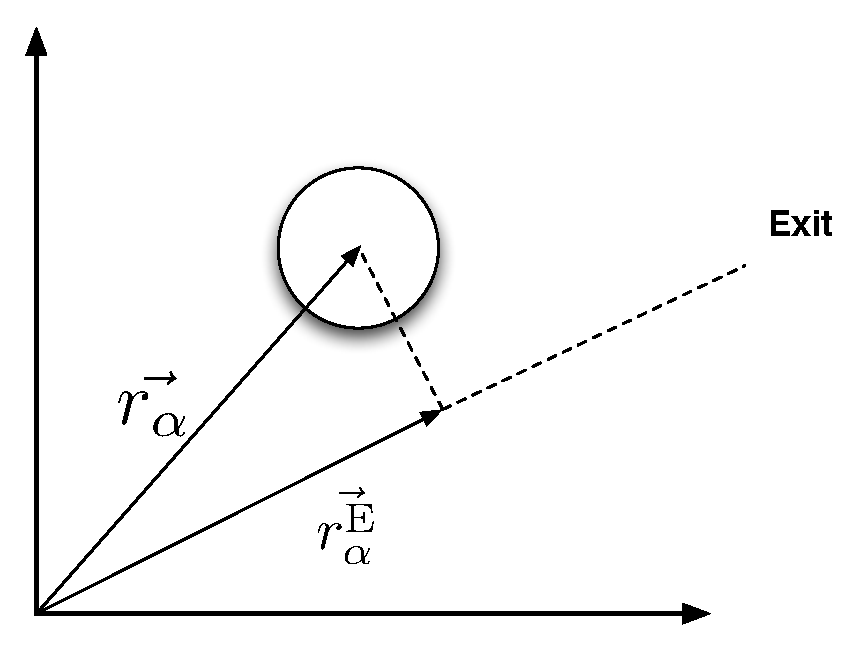
\includegraphics[scale=0.35]{Figures/NotationOfAgent2.pdf}} 
\caption{Illustration of the vector $ \vec{r_{\alpha}^{E}}$, which is the projection of $ \vec{r_{\alpha}} $ onto the desired direction of motion.}
\label{impatience}
\end{figure}

Therefore, we want to calculate $\overline{V}_{\alpha} \left( t \right)$ in the following way:
\begin{equation}\label{averagespeed}
   \overline{V}_{\alpha} \left( t \right) = \frac{1}{t} \vec{r_{\alpha}}\cdot \vec{e_{\alpha}} 
\end{equation}
\item From Equation \ref{v0eta} the initial desired speed $V_{\alpha}^{0} \left( 0 \right)$ is used to calculated desired speed at any time $ t $, and if we put $ t=0 $ into the equation, we have
\begin{equation}
    V_{\alpha}^{0}\left( 0 \right) = \left[ 1 - \eta_{\alpha} \left( 0 \right) \right] 
    V_{\alpha}^{0} \left( 0 \right) +
    \eta_{\alpha} \left( 0 \right)V_{\alpha}^{\text{max}}
\end{equation}
where $ \eta_{\alpha} \left( 0 \right) $ is not known.
Also for Equation \ref{eta}, put $ t=0 $ and we get
\begin{equation}
	\eta_{\alpha} \left( 0 \right) =
    1 - \frac{\overline{V}_{\alpha} \left( 0 \right)}
             {V_{\alpha}^{0} \left( 0 \right)}
\end{equation}
although the initial average speed $ \overline{V}_{\alpha} \left( 0 \right) $ is not defined in the original article, we decide to put $ \overline{V}_{\alpha} \left( 0 \right)=0 $, because in that case 
\begin{eqnarray}
	\eta_{\alpha} \left( 0 \right) &=&
    1 - \frac{\overline{V}_{\alpha} \left( 0 \right)}
             {V_{\alpha}^{0} \left( 0 \right)}\\
&=& 1 - \frac{0}{V_{\alpha}^{0} \left( 0 \right)}
= 1
\end{eqnarray}
which makes sense, as when the emergency suddenly happens our agent should feel extremely anxious ($ \eta_{\alpha} \left( 0 \right)=1 $). Then we know the initial desired speed $ V_{\alpha}^{0}\left( 0 \right) $ is
\begin{eqnarray}
    V_{\alpha}^{0}\left( 0 \right) &=& \left[ 1 - \eta_{\alpha} \left( 0 \right) \right] 
    V_{\alpha}^{0} \left( 0 \right) +
    \eta_{\alpha} \left( 0 \right)V_{\alpha}^{\text{max}}\\
&=& \left( 1 - 1 \right)  
    V_{\alpha}^{0} \left( 0 \right) +
    1 V_{\alpha}^{\text{max}}\\
&=& V_{\alpha}^{\text{max}}
\end{eqnarray}
\item Equation (\ref{v0eta}) and Equation (\ref{eta}) contains an intermediate variable $ \eta_{\alpha} \left( t \right) $, 
so in principle we are allowed to eliminate $ \eta_{\alpha} \left( t \right) $ and only show the 
relationship between $ V_{\alpha}^{0}(t) $ and $ \overline{V}_{\alpha} \left( t \right) $. Thus we get:

\begin{equation}\label{vv}
    V_{\alpha}^{0}(t) = \left[ 1 - \frac{V_{\alpha}^{max}}{V_{\alpha}^{0}(0)}\right]\overline{V}_{\alpha} \left( t \right) + V_{\alpha}^{max}
\end{equation}

\begin{figure}[ht]
\centering
{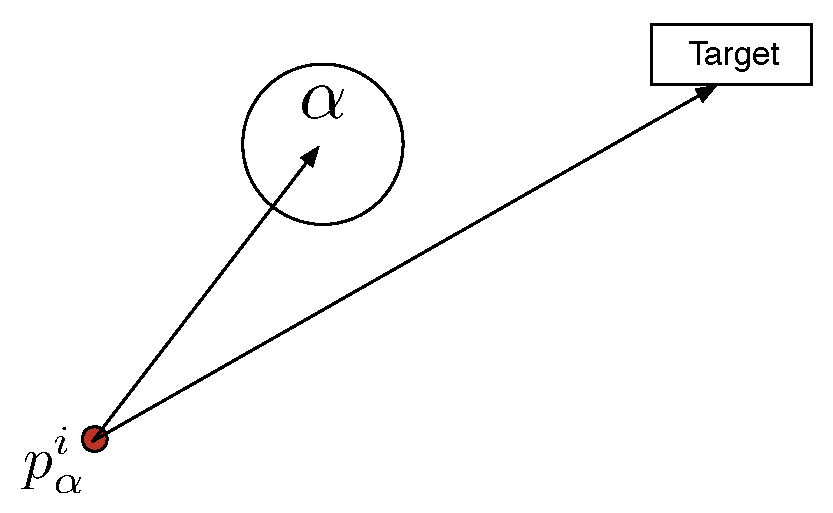
\includegraphics[scale=0.35]{Figures/impatience.pdf}} 
\caption[The impatience factor]{Illustration on the correlation between the function about the desired speed $ V_{\alpha}^{0}(t) $ 
and the average speed in the desired direction of motion $ \overline{V}_{\alpha} \left( t \right) $, and the graph of
$ V_{\alpha}^{0}(t) = \left[ 1 - \frac{V_{\alpha}^{max}}{V_{\alpha}^{0}(0)}\right]\overline{V}_{\alpha} \left( t \right) + V_{\alpha}^{max} $
intersects with the axis at $ \left( 0 , V_{\alpha}^{max} 
\right)  $ and $ \left(V_{\alpha}^{max} 
		\frac{V_{\alpha}^{0} \left( 0 \right) }{V_{\alpha}^{max}-V_{\alpha}^{0} \left(0 \right)} , 0 
\right)  $.
When $\alpha$'s velocity is at maximum the impatience gets low, and vice versa.}
\label{fig:impatience}
\end{figure}

Figure (\ref{fig:impatience}) is a drawing of the graph about those two variables, and the intersection
 of the function line with both axis are:

\begin{equation}
\left( 
	\overline{V_{\alpha}} , V_{\alpha}^{0} \left( t \right)
\right)
=
\left( 
	0 
		, 
	V_{\alpha}^{max} 
\right) 
\text{and} 
\left(
	V_{\alpha}^{max} 
		\frac{V_{\alpha}^{0} \left( 0 \right) }{V_{\alpha}^{max}-V_{\alpha}^{0} \left(0 \right)} 
	, 0 
\right) 
\end{equation}
Normally, the values of the two speeds should have positive values, so the graph is part of a straight line.
Now there is a doubt the range of the value of $ \overline{V}_{\alpha} \left( t \right) $, compared with $ V_{\alpha}^{max} $, 
if we have already 
set $ V_{\alpha}^{max} $ a fixed number for a certain agent. In the case:
\begin{equation}
	V_{\alpha}^{max} 
	\geq 
	V_{\alpha}^{max} 
	\frac{V_{\alpha}^{0}(0)}{V_{\alpha}^{max}-V_{\alpha}^{0}(0)}
\end{equation}
we get the relation:
\begin{equation}
V_{\alpha}^{0}(0)\leq \frac{1}{2} V_{\alpha}^{\text{max}}
\end{equation}
Which contradicts with our earlier conclusion that
\begin{equation}
    V_{\alpha}^{0}\left( 0 \right) = V_{\alpha}^{\text{max}}
\end{equation}
Therefore, the graph should not intersect with $ \overline{V_{\alpha}} $ axis under normal circumstances when the maximum desired velocity is not exceeded.
\item However, from Equation \ref{vv}  and Figure \ref{impatience} we think that $V_{\alpha}^{\text{max}}$ can be exceeded, but only under rare situations. For example, at $ t=0 $, if agent $ \alpha $ moves opposite to the exit because of some extreme large repulsive force, then from Equation \ref{vv} $ V_{\alpha}^{0} \left( 0 \right)  $ is larger than $V_{\alpha}^{\text{max}}$.
\item If there are no repulsive forces at all, the only source of acceleration is from the desired velocity, which modifies the actual velocity to the desired direction and value.  After some time, the actual velocity should reach some constant, which resembles the so called terminal velocity in physics when the acceleration is zero.  When the agent reaches the terminal velocity the actual velocity does not change and it equals the average velocity, so we can write the acceleration from Equation \ref{relaxtime} as

\begin{equation}
\vec{f}_{\alpha} = \vec{f^{0}_{\alpha}}\left( \vec{V_{\alpha}} \right)
\end{equation}
\begin{equation}
\frac{1}{\tau}\left( V_{\alpha}^{0} \vec{e_{\alpha}} - \overline{V}_{\alpha} \left( t\right) \vec{e_{\alpha}}  \right)  = 0
\end{equation}
As $ \tau $ is a constant, despite the direction of the velocity vector we have
\begin{equation}\label{terminal}
	 V_{\alpha}^{0} - \overline{V}_{\alpha} \left( t\right) 
    = 0
\end{equation}

Also we take Equation \ref{vv}, and insert the value of $ V_{\alpha}^{0}(t) $ from Equation \ref{vv} to Equation \ref{terminal}:

\begin{equation}
	\left[ \left( 1 - \frac{V_{\alpha}^{max}}{V_{\alpha}^{0}(0)}\right)\overline{V}_{\alpha} \left( t \right) + V_{\alpha}^{max} \right] - \overline{V}_{\alpha} \left( t\right) 
    = 0
\end{equation}
Solve for $ \overline{V}_{\alpha} \left( t\right) $ we get:
\begin{equation}
\overline{V}_{\alpha} \left( t\right) = V_{\alpha}^{0}(0)
\end{equation}
Which makes a lot of sense because the terminal velocity is the initial desired velocity and equals the maximum desired velocity.

\item The impatience or nervousness factor is active when one calculates the 
force action on agent $\alpha$ from the velocity of the agent.

In the case where $0 \leq \eta_{\alpha} \leq 1$ the expression for 
$V_{\alpha}^{0} \left( t \right)$  makes sense. Here we can see why this term 
is called the impatience of the agent. If the fraction  between the average 
speed in the desired direction and the initial speed is low then $\eta_{\alpha} \approx 1$. 
When the impatience term is close to one $V_{\alpha}^{0} \left( t \right)$ 
is dominated by $V_{\alpha}^{\text{max}}$. That is, if the agent have not 
moved very far in the desired direction compared to the initial speed the 
impatience of the agent will cause the agent's future velocity to be dominated by 
the desired velocity of the agent.

If the agent has been moving in the desired direction with his initial 
speed the entire time then $\eta_{\alpha} = 0$  and 
$V_{\alpha}^{0} \left( t \right)$ will continue to be $V_{\alpha}^{0} \left( 0 \right)$.

In the case where $\eta_{\alpha} \leq 0$ that is the agent has moved further 
in the desired direction then he would have had he been walking with his 
initial speed. The expression for $V_{\alpha}^{0} \left( t \right)$
stats yield strange results. That $\eta_{\alpha} \leq 0$ would imply that:

\begin{equation}\label{n}
    V_{\alpha}^{0} \left( t\right) = \left[ 1 + \eta_{\alpha} \left( t \right) \right] 
    V_{\alpha}^{0} \left( 0 \right) -
    \eta_{\alpha} \left( t \right)V_{\alpha}^{\text{max}}
\end{equation}

And this will yield a negative value for $V_{\alpha}^{0}$ if: 

\begin{equation}
\left[ 1 + \eta_{\alpha} \left( t \right) \right] 
V_{\alpha}^{0} \left( 0 \right) < \eta_{\alpha} \left( t \right)V_{\alpha}^{\text{max}} 
\end{equation}

This is a problem because it is not that far fetched that an agent will be 
forced to exceed his desired velocity.

In the case where $1 \leq \eta_{\alpha}$ it would mean that the agent has moved 
further in the opposite direction than the desired one and this can only happen very 
weird situations.
\end{itemize}

% Lets have a little summation here. What have we learned about the inpatience factor and
% the velocity dependant force. What kind of dynamics does this force yield





\subsubsection{Repulsion from the walls}
Now the second term on the right hand side of \eqref{model} is a force which arise from interactions with the walls or other obstacles. The forces, caused by the wall or obstacles, is given by:

\begin{equation}\label{wallpotential}
    \vec{f_{\alpha B}} \left( \vec{r_{\alpha}} \right) =
    - \nabla_{\vec{r_{\alpha}}} U_{B}
    \left( \| \vec{r_{\alpha}} - \vec{r_{B}^{\alpha}} \| \right)
\end{equation}
$U_B$ is a repulsive potential and $ \| \vec{r_{\alpha}} - \vec{r_{B}^{\alpha}} \|$ is the distance 
from the position of agent $\alpha$ to the nearest point $ \vec{r_{B}^{\alpha}}  $ of the wall and shown in figure \ref{NotationOfWall}.

\begin{figure}[ht]
\centering
{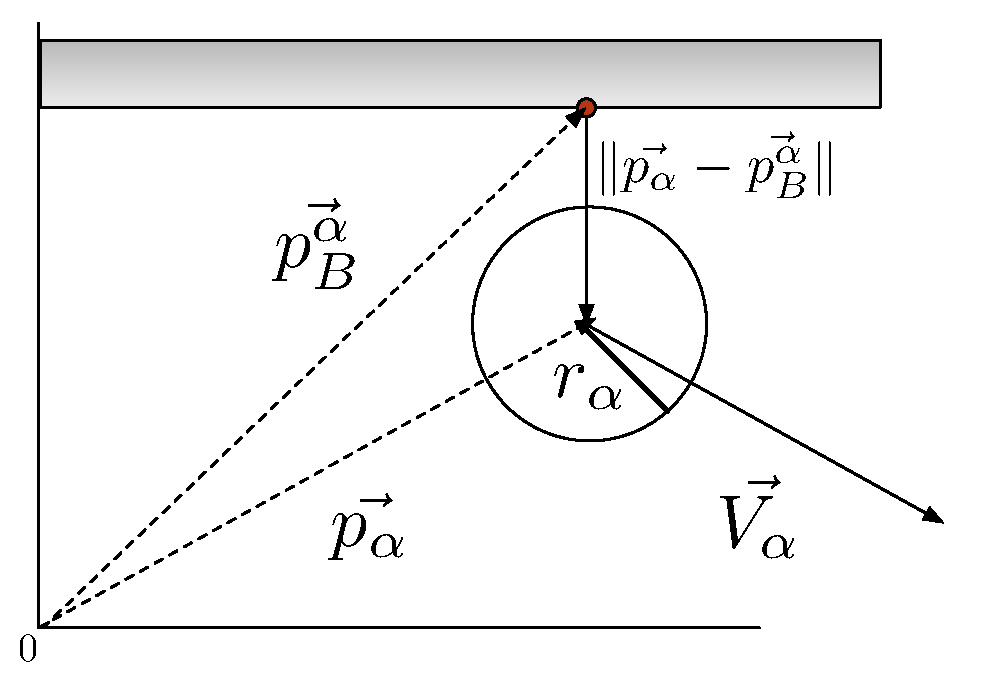
\includegraphics[scale=0.35]{Figures/NotationOfWall.pdf}} 
\caption[Notation of the interaction between an agent and a wall]{The illustration shows the mathematical notation for the interaction with walls used. The circle is pedestrian $\alpha$ with radius $r_{\alpha}$, $\vec{r_{\alpha}}$ is the position vector for $\alpha$, the grey box on the top is the wall, $\vec{r_{B}^{\alpha}}$ is the position vector for the closest part of the wall to $\alpha$, $\left( \| \vec{r_{\alpha}} - \vec{r_{B}^{\alpha}} \| \right)$ is the smallest distance from $\alpha$ to the wall and $\vec{V_{\alpha}}$ is the velocity vector for $\alpha$.}
\label{NotationOfWall}
\end{figure}

\begin{itemize}
\item  $U_B$ only depends on the distance $ \| \vec{r_{\alpha}} - \vec{r_{B}^{\alpha}} \|$, so the gradient of $V_B$ tells us in which direction does this distance change the most. It is obvious that the changes is largest if the agent takes a step directly towards or away from the wall, which means that the agent will always be pushed directly away from the wall.

\item The next job is to find an explicit expression for $ \| \vec{r_{\alpha}} - \vec{r_{B}^{\alpha}} \|$\\
To start of with we need to find point on the wall that is perpendicular to $\alpha$ as it will be the nearest.  
If we define the wall as a vector, $\vec{W}$ going from a point in space $w_1$ to another point $w_2$, then we can find the projection of $\alpha$ onto the wall and this projection will be $\vec{r_{B}^{\alpha}}$.
The equation for the projection is
\begin{equation}\label{wall}
\vec{r_{B}^{\alpha}}=\frac{\vec{r_{\alpha}}\cdot \vec{W}}{\| \vec{W} \|^2}\vec{W}
\end{equation}
With this we now have the two points we need to calculate $ \| \vec{r_{\alpha}} - \vec{r_{B}^{\alpha}} \|$.


\item With the explicit expression for $ \| \vec{r_{\alpha}} - \vec{r_{B}^{\alpha}} \| $, we are able to calculate $ \vec{f_{\alpha B}} \left( \vec{r_{\alpha}} \right) $ from Equation \ref{wallpotential}, if the expression for the potential function $ V_{B}
    \left( \| \vec{r_{\alpha}} - \vec{r_{B}^{\alpha}} \| \right) $ is given.\\
In some of the other articles [ ] made by the same outhers as the article which makes the basis for the model in this repport, the repulsive potential from the wall is given as
\begin{equation}
U_{B} \left( \| \vec{r_{\alpha}} - \vec{r_{B}^{\alpha}} \| \right) =
U^0_{\alpha B} e^{- \| \vec{r_{\alpha}} - \vec{r_{B}^{\alpha}} \| / r_{\alpha} }
\end{equation}
where $U^0_{\alpha B}$ is a constant and $r_{\alpha}$ is the radius of a pedestrian $\alpha$. \\

In that case, the wall repulsive force on agent $ \alpha $ is:
% TODO: make \begin{equation} and \begin{slpit}. This is a general thing for all \begin{allign}
\begin{equation}
    \vec{f_{\alpha B}} \left( \vec{r_{\alpha}} \right) =
    - \nabla_{\vec{r_{\alpha}}} U_{B}
    \left( \| \vec{r_{\alpha}} - \vec{r_{B}^{\alpha}} \| \right)\\
=-\left( \frac{\partial}{\partial x_{\alpha}}U_{B}( \| \vec{r_{\alpha}} - \vec{r_{B}^{\alpha}} \|), \frac{\partial}{\partial y_{\alpha}}U_{B}( \| \vec{r_{\alpha}} - \vec{r_{B}^{\alpha}} \|)\right) \\
\end{equation}
Calculating the derivatives we get 
\begin{equation}
    \vec{f_{\alpha B}} \left( \vec{r_{\alpha}} \right) 
=-\left(\left(U^0_{\alpha B}\frac{1}{r_{\alpha}}\frac{e^{- \| \vec{r_{\alpha}} - \vec{r_{B}^{\alpha}} \| / r_{\alpha} } (x_{\alpha}-x_B^{\alpha})}{\| \vec{r_{\alpha}} - \vec{r_{B}^{\alpha}} \| }\right),\left(U^0_{\alpha B}\frac{1}{r_{\alpha}}\frac{e^{- \| \vec{r_{\alpha}} - \vec{r_{B}^{\alpha}} \| / r_{\alpha} } (y_{\alpha}-y_B^{\alpha})}{\| \vec{r_{\alpha}} - \vec{r_{B}^{\alpha}} \| }\right)\right) \\
\end{equation}

\item The exponential function will always lay between 0 and 1:
\begin{equation}
0 < e^{ -\| \vec{r_{\alpha}} - \vec{r_{B}^{\alpha}} \| /r_\alpha} < 1
\end{equation}
Which leads to
\begin{equation}
0< U_{B} \left( \| \vec{r_{\alpha}} - \vec{r_{B}^{\alpha}} \| \right) < U^0_{\alpha B}
\end{equation}
We can see that this force act in the following way:\\
$\vec{f_{\alpha B}}$ tends to 0 as the distance $ \| \vec{r_{\alpha}} - \vec{r_{B}^{\alpha}} \|$ gets large, meaning that a pedestrian in a reasonably distance from the wall will feel a diminishing force. $\vec{f_{\alpha B}}$ tends to $V^0_{\alpha B}$ as the distance $ \| \vec{r_{\alpha}} - \vec{r_{B}^{\alpha}} \|$ tends to $0$ the pedestrian will be pushed, with some force depending on $V^0_{\alpha B}$, away from the wall. 
The negative of the force means that when the potential between wall and pedestrian rises so will the force, but in the opposite direction meaning that the pedestrian will be pushed away. This can be understood as if the pedestrian is trying to avoid the wall as it is expected from real life situations.
 [Helbing and Molnár, 1995]. %real references, please.
\end{itemize}

 
\subsubsection{Repulsion from other agents}
The third term on the right hand side of \eqref{model} is a summation of all the 
force between agent $\alpha$ and agent $\beta$. It is a function of the position vector and the velocity of 
both agents, and it is given by:

\begin{equation}
    \sum_{\beta \left( \neq \alpha \right)}
        \vec{f_{\alpha \beta }}\left( t \right) =
        A_{\alpha}^{1} exp \left(
            \frac{ r_{\alpha \beta} - d_{\alpha \beta }}
                 {B_{\alpha}^1}
        \right)
    \vec{\eta_{\alpha \beta}} \cdot
    \left(
        \lambda_{\alpha} + \left(
            1 - \lambda_{\alpha}
        \right)
		\frac{1+\cos{\phi}}{2}
    \right) +
    A_{\alpha}^{2} exp\left(
        \frac{r_{\alpha \beta} - d_{\alpha \beta}}
             {B_{\alpha}^{2}}
    \right)
    \vec{\eta_{\alpha \beta}}
    \label{agentinteraction}
\end{equation}

\begin{figure}[ht]
    \centering
    {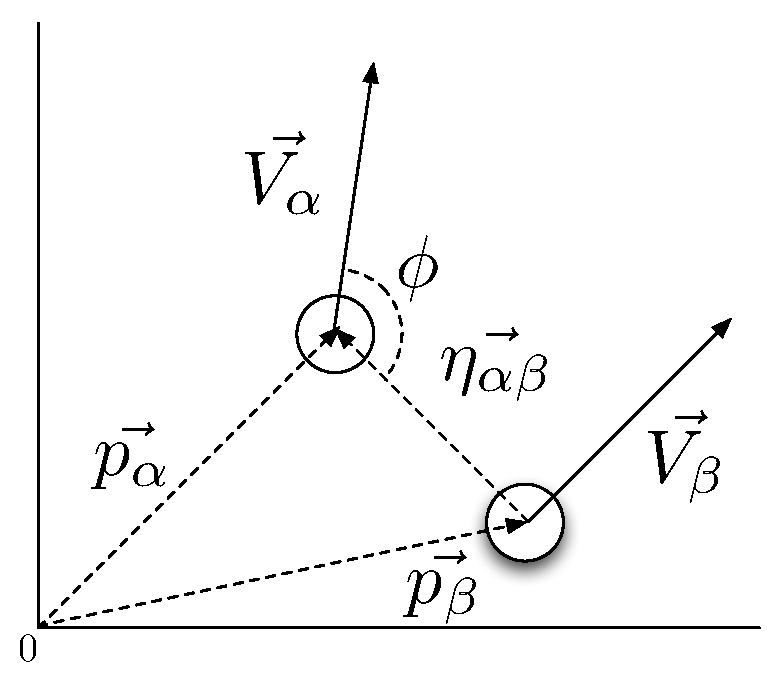
\includegraphics[scale=0.35]{Figures/NotationOfInteraction.pdf}} 
    \caption[Notation of the interaction between two agents]{Illustration of the notation for the interaction between agents.
	     An addition and difference to \ref{NotationOfWall} is that the wall has been replaced by pedestrian $\beta$.
	     $\eta_{\alpha \beta}$ is the normal vector pointing from $\alpha$ to $\beta$, and $\phi$ is the angle between $\alpha$'s 
	     velocity vector and $\beta$'s center of mass.}
    \label{NotationOfInteraction}
\end{figure}

Here $A_{\alpha}^{1}$, $A_{\alpha}^{2}$, $B_{\alpha}^{1}$, $B_{\alpha}^{2}$ 
and $\lambda_{\alpha}$ are all constants that can differ for each agent. 
$r_{\alpha \beta}$ is the sum of the radii of $\alpha$ and $\beta$ that is 
$r_{\alpha \beta} = r_{\alpha} + r_{\beta}$. $d_{\alpha \beta}$ is the 
distance from the center of mass of agent $\alpha$ and the center of mass of 
agent $\beta$ and is therefore given by $d_{\alpha \beta} = 
\|\vec{r_{\alpha}}\left( t \right) - \vec{r_{\beta}}\left( t \right) \|$.
$\eta_{\alpha \beta}$ is the normal vector pointing from $\alpha$ to $\beta$ 
and it is given by:

\begin{equation}
    \eta_{\alpha \beta} =
        \frac{\vec{r_{\alpha}}(t) - \vec{r_{\beta}}(t)}
             {\|\vec{r_{\alpha}}(t) - \vec{r_{\beta}}(t) \|}
\end{equation}

the angle $\phi$ in \eqref{agentinteraction} is the angle between the normal 
vector pointing from agent $\beta$ to $\alpha$ and the direction in which 
agent $\alpha$ is moving. Cosine to the angle is 

\begin{equation}
\cos \left( \phi \right)
	\left( t \right) 
		= 
	- \vec{\eta_{\alpha \beta}}
		\left( t \right) 
	\cdot 
\vec{e_{\alpha}}\left( t \right)
\end{equation}

Equation \eqref{agentinteraction} is divided into two terms. The first term on 
the right hand side reflects the agents tendency to stay at a certain distance 
from other agents. This part of the force is called the private sphere because 
the agent prefers to have some free space around him if possible. The radius 
of the private sphere can differ from agent to agent. The constant 
$A_{\alpha}^{1}$, $B_{\alpha}^{1}$ and $\lambda_{\alpha}$ control the nature 
of the private sphere $A_{\alpha}^1$ and $B_{\alpha}^1$ control the strength 
and range of the interaction respectively. $\lambda_{\alpha}$ is there to take 
into account a persons tendency to focus on things happening in front of him 
rather than behind him.	% we should make a drawing of this.

The second term of equation \eqref{agentinteraction} deals with physical interaction.
In the situation where the density of the crowd is high the agents will have be closer
to each other and the social sphere is undermined. % go more into detail here 
So if we look away from the social sphere for a minute and concentrate on the physical
interaction we will see that if we omit the social sphere the calculation will be reduced to
to:

\begin{equation}\label{re}
\overrightarrow{f_{\alpha\beta}}(t) = A_{\alpha}^{2} exp\left[ \frac{r_{\alpha\beta} - d_{\alpha}\beta}{B_{\alpha}^{2}}\right]  \overrightarrow{n_{\alpha\beta}}
\end{equation}

Taking the norms of both sides of Equation (\ref{re}), we can draw the relation between the value of $\overrightarrow{f_{\alpha\beta}}(t)$ and $ d_{\alpha\beta} $, as shown in Figure 
(\ref{physicalinteraction}).\\

\begin{figure}
    \centering
    {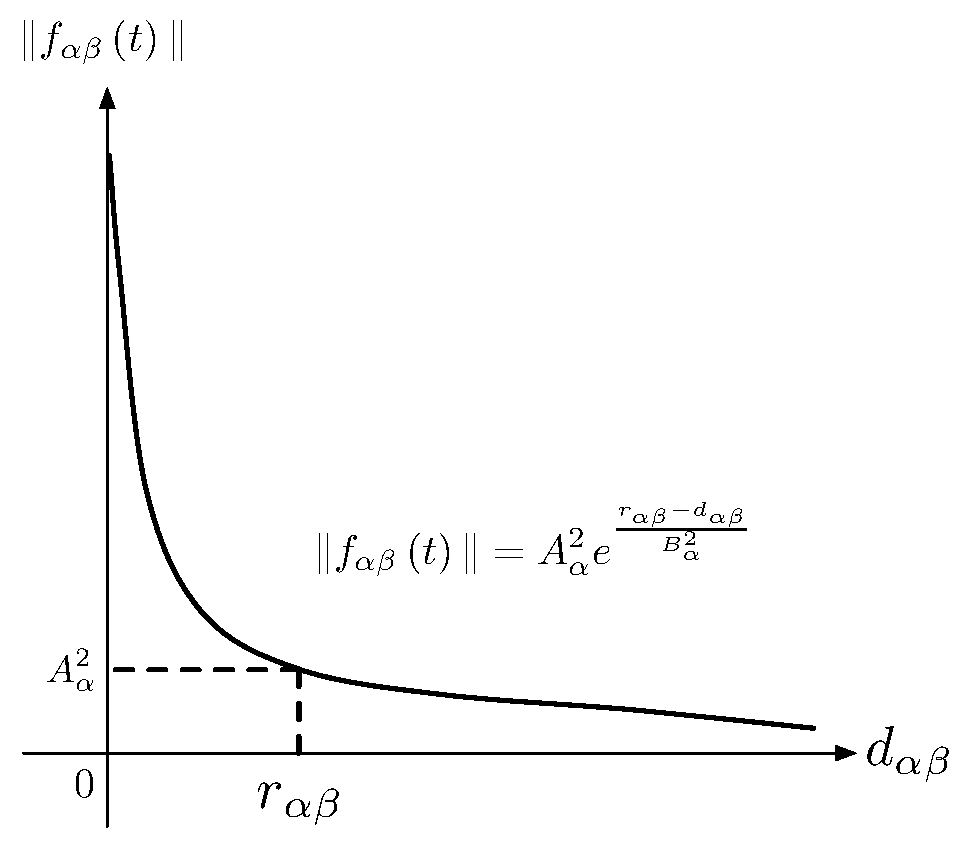
\includegraphics[scale=0.45]{Figures/physicalinteraction.pdf}} 
    \caption[Psysical interaction]{Illustration of the function about the interaction force 
        $f_{\alpha\beta}(t)$ and the distance between two agents
        $d_{\alpha \beta}$. It follows that the smaller the distance between two agents, the greater the interaction force is. }
    \label{physicalinteraction}
\end{figure}

There is one intersection of the graph and the  axis at:

\begin{equation}
	\left( d_{\alpha \beta} , \| \vec{f_{\alpha \beta}} \left( t \right) \| \right)
 =
	\left( 0 , A_{\alpha}^{2} exp\left( \frac{r_{\alpha\beta} }{B_{\alpha}^{2}}\right)  \right) 
\end{equation}

If put into the constants, we will be able to get a maximum value of $ f_{\alpha\beta}(t) $, 
since the distance between agents cannot be negative. Here we set $ A_{\alpha}^{2} = 3 m/s^{2} $, 
$ r_{\alpha\beta} = 0.6 m $, and $ B_{\alpha}^{2} = 0.2 m $, so 
$ f_{\alpha\beta}(t)^{max} \doteq 60 m/s^{2} $, which is about six times the gravitational 
acceleration and represents a rather large force between agents (as large as six person's weight).

However, we notice that the effective part of the force calculated above is only the horizontal 
component that enables the agent to move horizontally in the plane where we do the simulation, 
but the reality is that the agents sometimes are also able to move vertically, for example, 
by stepping upon other people when they cannot take the pushing force from the surrounding agents. 
When that happens, the horizontal component of the repulsive force becomes smaller even if $ d_{\alpha\beta} $ 
is kept the same.	

\begin{figure}[ht]   
\centering
    {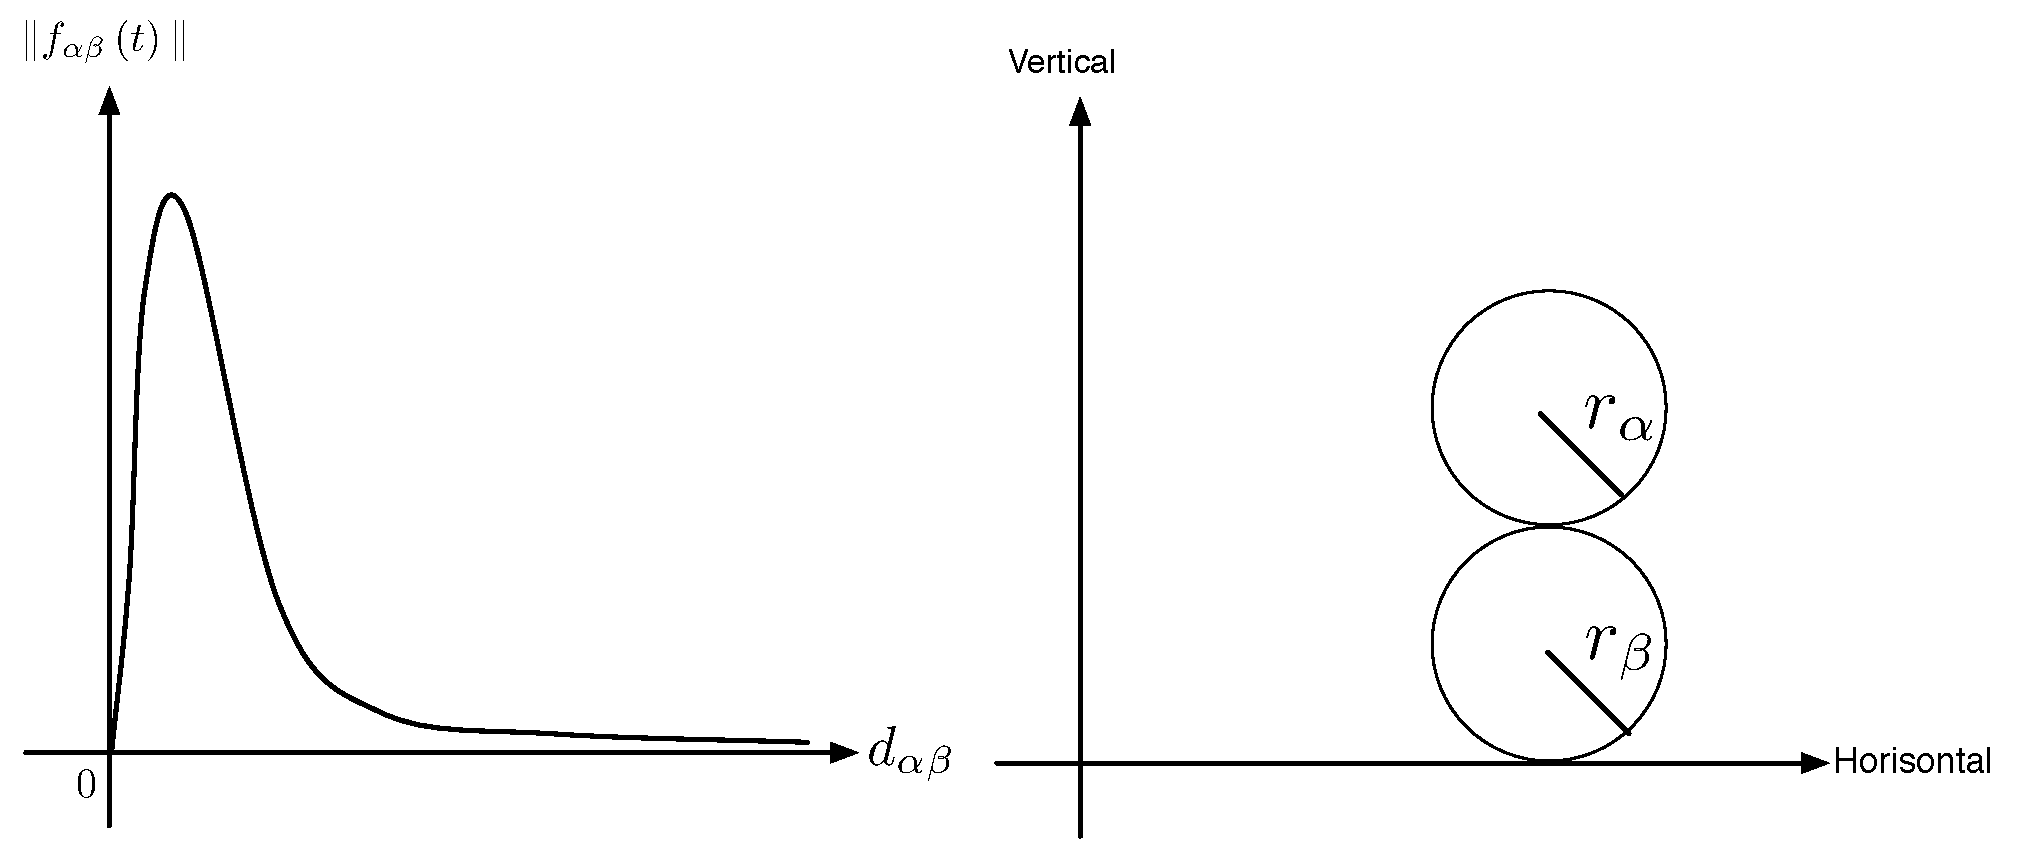
\includegraphics[scale=0.35]{Figures/ForceOverlapping.pdf}} 
    \caption{}
    \label{forceoverlapping}
\end{figure}

Therefore, a qualitative modification of dependence between $ f_{\alpha\beta}(t) $ and $ d_{\alpha\beta} $ could be:
% remember to finish this section

% again lets  have a little summation here. What kinds of dynamics does the
% social interaction part of the model yield.

\subsubsection{The attractive forces between some agents}
The fourth and last term in \eqref{model} represents the force from attraction 
in the room. Attractions can be either be either interesting sculptures or 
sights or familiar persons the agent prefer to be close to, such as friends 
and family. The mathematical structure of this force is the same as the force 
from other agents, however it is opposite in algebraic sign and has different 
constants. 

To get an overview of how the model is put together look a figure \ref{overview}
with the aid of table \ref{tableofconstandvar}

\begin{figure}[hb] %with some more comments i think that this figure could serve as a summation of the entire section
    \centering
    {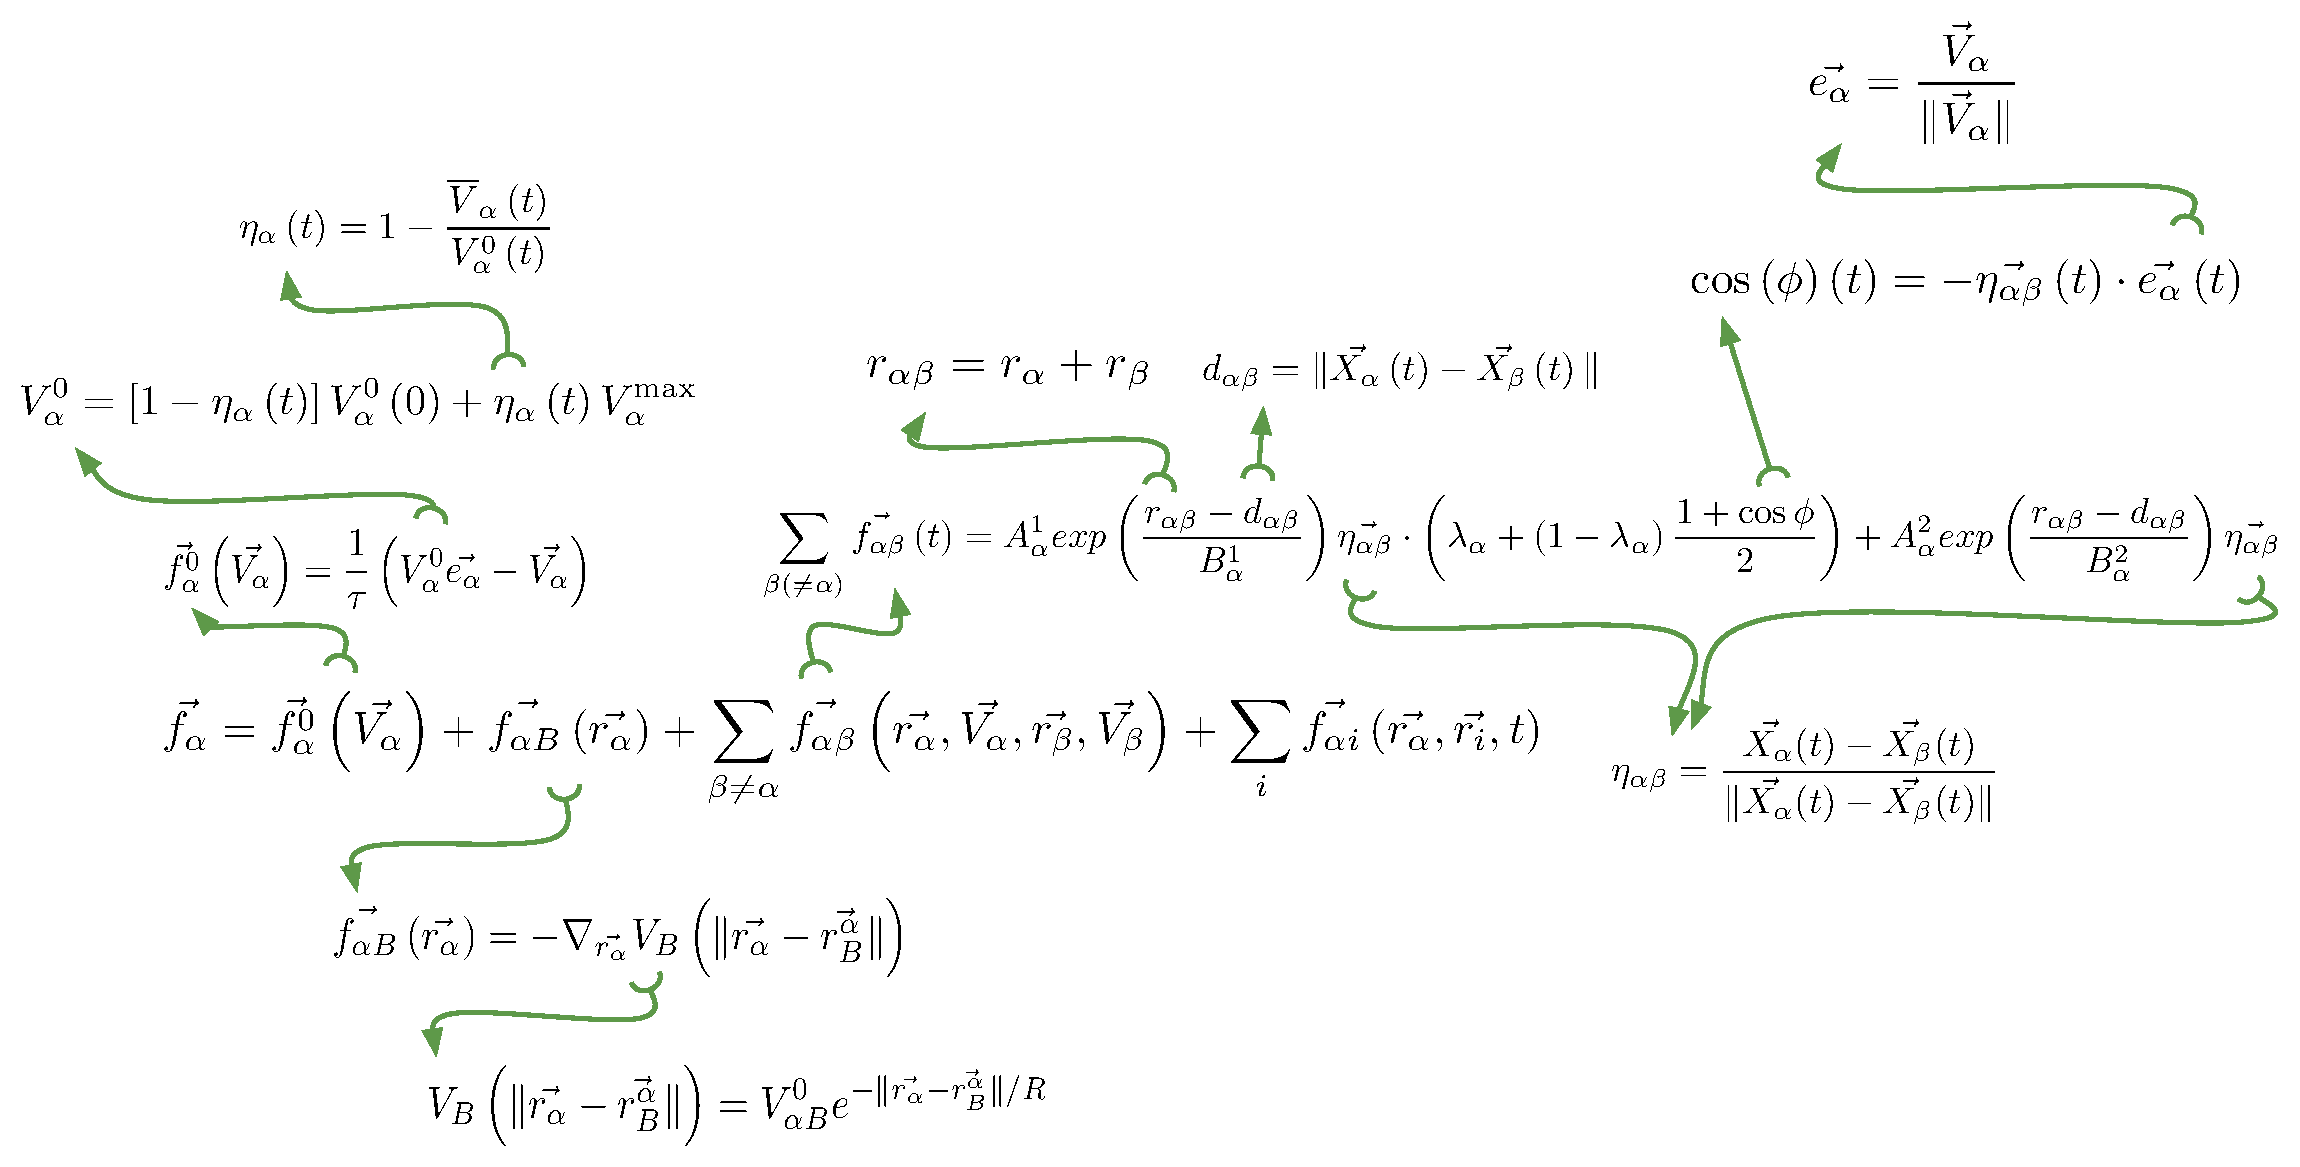
\includegraphics[scale=0.45]{Figures/overview.pdf}} 
    \caption[Overview of the model]{Illustration of an overview of how the model is put together. The different equations and their notation is written to give the 
	     reader an overview of how the model looks like.}
    \label{overview}
\end{figure}
\clearpage
\section{sec:discussion}\label{sec:discussion}
\subsection{Repulsive force}
In chapter 3 we have seen the formulas for calculating the repulsive forces from the wall and other agents are very similar, both are exponential functions decreasing with some distance, which makes us wonder if both come from the same origin.\\

\begin{itemize}
\item The difference between those two repulsive forces is basically one is from a single point and the other is from an object that has a dimension much larger than a single agent. If we imagine our agents are particles with negative charge, then there is a pair of repulsive forces which has direction along the line connecting the two particles and magnitude depending on the distance between them. Further we can put lots of particles along a bar, see Figure
Summing up all the repulsive forces from each particle on the bar will give the repulsive force that the charged bar on the single particle $\alpha$.

\item Applying the idea above to analyse our wall repulsion, as a simple start we place the agent $\alpha$ a distance $ d $ away from the wall which as a length $L$, and by symmetry we know the resulting force must point vertically downwards, see Figure.\\

Integrating the forces can be written as:

\begin{equation}\label{integ}
\vec{f_{\alpha B}} = 
\int_0^L \! \vec{f_{\alpha\beta}} \, \mathrm{d}l
\end{equation}

\item When the repulsive force is known, the expression for the wall potential can be calculated, which can be done by integrating the force along a path. Normally the potential at some position is defined as the work done on the particle by that potential field when the particle is moved from that position to infinitely far away.

\begin{equation}\label{pot}
	U_{B}= \int_{\vec{r_{\alpha}}�}^{text{f}\infty} \! \vec{f_{\alpha B}} \cdot \, \text{d}\vec{r_{\alpha}} 
\end{equation}

\item In some article [Helbing 2000], the repulsive force from the wall is given by:
\begin{equation}\label{helbing2000}
\vec{f_{\alpha B}} = 
	\left( 
			\left[ 
	A exp 
				\left[ 
						\left(  
							r_{\alpha}-d_{\alpha B}
						\right)  / B
				\right] +kg 
					\left( 
						r_{\alpha}-d_{\alpha B} 
					\right) 
			\right] 
		\right)
	\vec{n_{B}^{\alpha}}-\kappa g 
	\left(
		r_{\alpha}-d_{\alpha B}
	\right) 
	\left(
			\vec{V_{\alpha}}\cdot \vec{t_{iw}}
	\right) 
\vec{t_{iw}}
\end{equation}

where $ r_{\alpha} $,  $ \vec{V_{\alpha}} $ are the radius and velocity of agent $ \alpha $ as we noted before, $ A $, $ B $, $ k $, $ \kappa $ are constants, $ d_{\alpha B} $ is the distance from the agent to the wall, $ \vec{n_{B}^{\alpha}} $ is a normal vector from the wall, $ \vec{t_{iw}} $ is a tangent vector to the wall. $ g $ is a function of some variable.\\
In this expression, the wall repulsion force to agent $ \alpha $ is not always perpendicular to the wall, but the force has two components, one perpendicular to the wall and the other tangent to the wall. Particularly the tangent component depends on the velocity of $ \alpha $. However, in Helbing's latest articles he does not show the expression of Equation \ref{helbing2000}, but use the gradient of potential instead. 
\end{itemize}


\subsection{The repulsive force between agents in $ \Re ^{3}$}
From the given formula for calculating the repulsive force between agents in the description of the model, the part calculating the force to keep the personal space can be omitted when the agents are rather close to each other, then the calculation can be reduced as Equation (\ref{eq:re}).

\begin{equation}\label{eq:re}
\overrightarrow{f_{\alpha\beta}}(t) = A_{\alpha}^{2} exp\left[ \frac{r_{\alpha\beta} - d_{\alpha}\beta}{B_{\alpha}^{2}}\right]  \overrightarrow{n_{\alpha\beta}}
\end{equation}

Taking the norms of both sides of Equation (\ref{eq:re}), we can draw the relation between the value of 
$\overrightarrow{f_{\alpha\beta}}(t)$ and $d_{\alpha \beta}$, as in Figure (\ref{fig:physicalinteraction})
\\
\begin{figure}
\centering
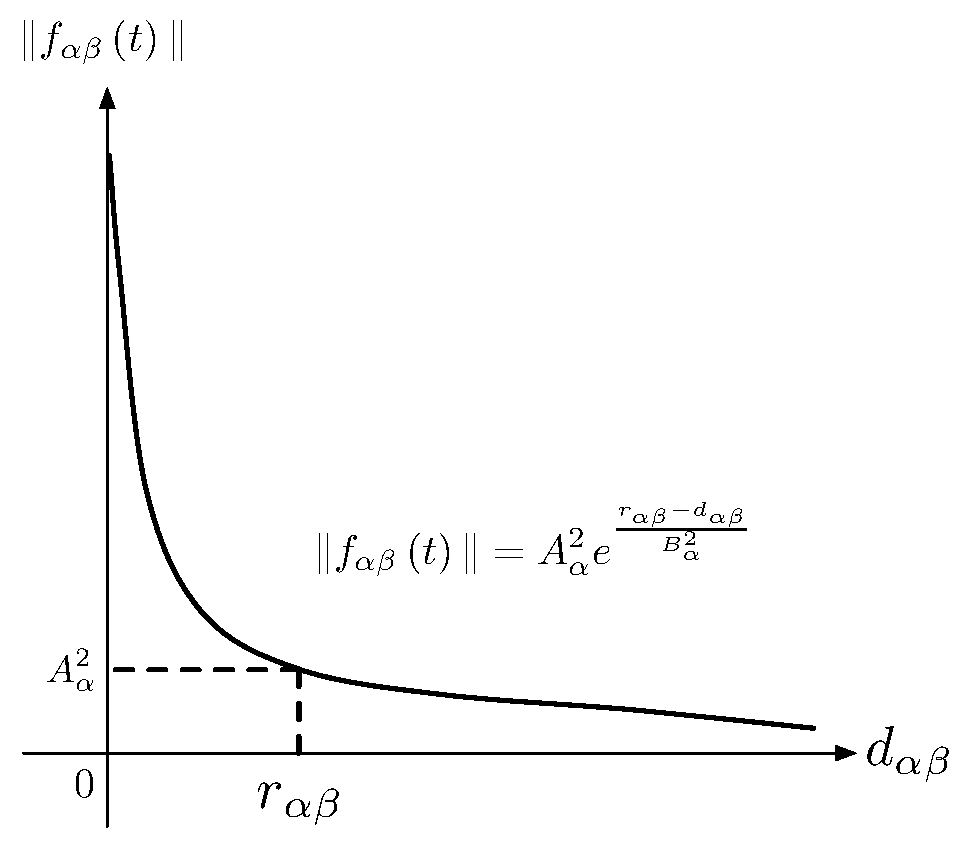
\includegraphics[scale=0.45]{Figures/physicalinteraction.pdf} 
\caption{The function about the interaction force $\vec{f_{\alpha\beta}}(t)$ and the distance between two agents
$d_{\alpha\beta}$ }\label{fig:physicalinteraction}
\end{figure}

There is one intersection of the graph and the axis $ \left( 0, A_{\alpha}^{2} exp\left( \frac{r_{\alpha\beta} }{B_{\alpha}^{2}}\right)  \right)  $. If put into the constants, we will be able to get a maximum value of $ f_{\alpha\beta}(t) $, since the distance between agents cannot be negative. Here we set $ A_{\alpha}^{2} = 3 m/s^{2} $, $ r_{\alpha\beta} = 0.6 m $, and $ B_{\alpha}^{2} = 0.2 m $, so $ f_{\alpha\beta}(t)^{max} \doteq 60 m/s^{2} $, which is about six times the gravitational acceleration and represents a rather large force between agents (as large as six person's weight). \\\\
However, we notice that the effective part of the force calculated above is only the horizontal 
component that enables the agent to move horizontally in the plane where we do the simulation, 
but the reality is that the agents sometimes are also able to move vertically, for example, 
by stepping upon other people when they cannot take the pushing force from the surrounding agents. 
When that happens, the horizontal component of the repulsive force becomes smaller even if 
$d_{\alpha\beta}$ is kept the same.	
Therefore, a qualitative modification of dependence between $ f_{\alpha\beta}(t) $ and $ d_{\alpha\beta} $ could be:
\begin{figure}[hb]   
\centering
    {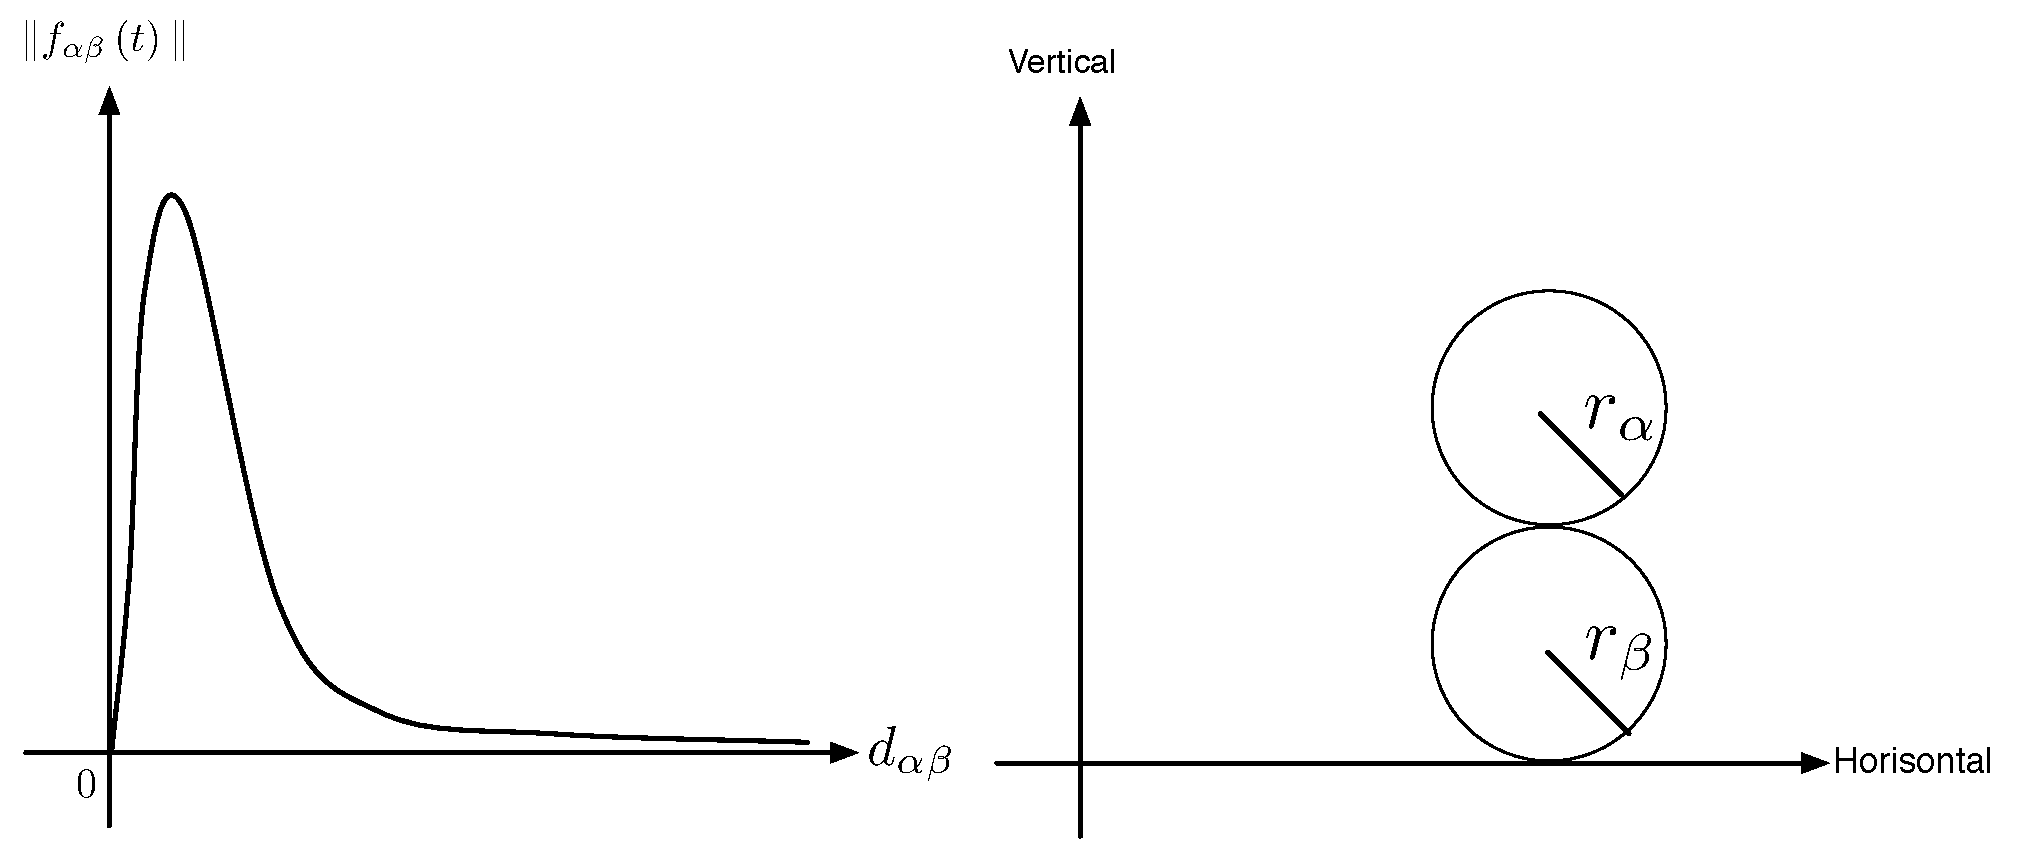
\includegraphics[scale=0.35]{Figures/ForceOverlapping.pdf}} 
    \caption{}
    \label{forceoverlapping}
\end{figure}
\\
\subsection{Use social force in further calculation}
use the value of forces to predict, as they are partly not real forces, the measurement does not reflect the reality in some range.
Pressure
\clearpage
% vim:ft=tex
\section{Simulation approach}
\label{sec:simulation}
In this section, we describe how our simulation is implemented, and how the 
implementation works. This is done in part to document our implementation, and 
in part to give the reader an overview of how our results are obtained.
We will describe briefly how the program is structured on a macro level, and 
go into more detail on the parts specific to the calculations of the model 
parameters. The full source code is available online\footnote{See 
\url{http://akira.ruc.dk/~tohojo/crowd-modelling}.}.

Our simulation is implemented in the Python programming language, with the 
calculation intensive parts implemented in C for performance reasons. We 
assume a virtual coordinate system using meters as a base unit, and with the 
origin in the centre of the area we simulate. Each pedestrian is 
described by a centre point and a radius, and each wall is described by a line 
segment connecting two points.

All parameters are stored as double precision floating point values where 
nothing else is indicated. We use custom data structures to keep track of the 
pedestrians and walls while running the simulation. Python is used to set up the 
initial conditions, run the program's main control loop, and draw the 
simulation results through the \emph{PyGame} library \cite{pygame}. This 
allows to do real-time animation as well as saving each simulation step 
to be assembled into a film afterwards. All calculations and data processing 
is done in a Python extension written in C, to increase performance. Gathering 
of data to draw the graphs and the drawing itself is done in the Python code. 

\subsection{Structure of the program}
The program is structured into four main parts: The simulation calculations, 
drawing of the simulations, plotting of parameters and the control part 
setting up parameters and calling the other parts as necessary. The drawing 
part mainly consists of a frontend to the drawing library, and so is not 
interesting to discuss here. The other parts will be described in the 
following, structured so as to present the sequence that is followed when a 
simulation is run. This description consists of three parts: setting up the 
simulation, calculations, and gathering of results.

\subsection{Setting up the simulation}
The program supports defining multiple \emph{scenarios} to simulate. Each 
scenario defines its own set of parameters, and a simulation run features one 
scenario. The parameters defined for each scenario include:

\begin{itemize*}
    \item The model constants, $A$, $B$, $U$, $\lambda$ and pedestrian relaxation 
        time. These are the same for all pedestrians in a simulation.
    \item Mean initial desired velocity and radius of pedestrians and their standard 
        deviation, and the factor used to calculate the maximum velocity.
    \item The initial number of pedestrians, the area(s) they start in and the 
        target(s) they move towards.
    \item The geometry of the scenario (i.e. placement of walls).
    \item Definition of the areas where measurement of data for plotting 
        graphs is done and which parameters should be plotted (see 
        section~\ref{sec:measurement}).
    \item Various parameters related to drawing of the simulation, maximum run 
        time and optional continuous inflow of pedestrians.
\end{itemize*}

Parameters that are not set for each scenario, but are defined once for all 
simulations are:

\begin{itemize*}
    \item Time step size.
    \item Plotting data sampling frequency.
\end{itemize*}

How the values of the parameters are determined is described in 
section~\ref{sec:init-cond}. From these parameters, the simulation is set up 
by initialising the calculation module and creating the pedestrians.

The pedestrians are created with an initial velocity of zero, and distributed 
randomly within the area(s) designated by the parameters for the scenario, as 
described in section~\ref{sec:init-pedestrians}. 

\subsection{Calculation of the model}
\label{sec:model-calculation}
For each step of the simulation, the calculations are run in two parts: 
Finding the accelerations (or resulting force) for all pedestrians, and 
updating position and velocity for the pedestrians.  Since the acceleration 
for each pedestrian is dependent on both position and velocity of the other 
pedestrians, splitting the calculations this way enables us to do the 
calculations of pedestrians in any order, and even parallel. The drawback 
is that the pedestrians are only affected by the movement and positions of 
other pedestrians as they were at the end of the last simulation step. This 
means that the time step has to be small enough that this doesn't matter in 
practice.

The acceleration vectors for each pedestrian, $\alpha$, is calculated in three 
steps, corresponding to the parts $\overrightarrow{f_\alpha^d}$, 
$\overrightarrow{f_{\alpha \beta}}$ and $\overrightarrow{f_{\alpha \gamma}}$ from 
section~\ref{sec:the-model}. In each simulation step the three forces are 
calculated in order, first calculating the desired force, then the repulsive 
force from each of the other pedestrians in the simulation, and finally the 
repulsive force from each wall. The resulting vectors are added to yield the 
total acceleration for each pedestrian.

After this is calculated for all pedestrians, their velocities and positions are 
updated in separate steps. Each of these four steps are described in detail 
in the following. The code calling the other parts of the calculation can be 
seen in code segment~\ref{lst:calling}. This function is called once for each 
pedestrian (index \texttt{i}) for each simulation step.

\begin{lstlisting}[caption={Main function calling the other parts of the 
    calculation code.},label=lst:calling]
void calculate_forces(Py_ssize_t i)
{
    int j;
    add_desired_acceleration(&pedestrians[i]);

    for(j = 0; j < a_count; j++) {
        if(i == j) continue;
        add_repulsion(&pedestrians[i], &pedestrians[j]);
    }

    add_wall_repulsion(&pedestrians[i]);
}
\end{lstlisting}

\subsubsection{Calculating the desired force}
The function for calculating the desired force can be seen in code 
segment~\ref{lst:desired-force}. Of note is the implementation on lines 7-19 
of the conditional definition of $V_\alpha^d(t)$ given in 
equation~\eqref{eqn:cond-define} and the creation of a unit vector in lines 
20-21 to add the direction to the desired velocity.

To increase performance, it is preferred to update values in place, instead of 
copying them around in different parts of the computer's memory. This gives 
rise to the constructs around the \texttt{vector\_i*}-functions in the code; 
here the \emph{i} stands for ``in place''.

\begin{lstlisting}[caption={Calculating the desired 
    force.},label=lst:desired-force]
static void add_desired_acceleration(Pedestrian * a)
{
    double average_velocity = 0.0, impatience = 0.0, 
           desired_velocity = 0.0;
    Vector desired_direction = {0.0, 0.0};

    if(a->time) {
        double proj = vector_projection_length(
                a->initial_position, a->target, a->position);
        average_velocity = proj / a->time;

        impatience = 1.0 - average_velocity / a->initial_desired_velocity;

        desired_velocity = (1.0-impatience) * a->initial_desired_velocity + \
                           impatience * a->max_velocity;

    } else {
        desired_velocity = a->initial_desired_velocity;
    }
    desired_direction = vector_sub(a->target, a->position);
    vector_unitise(&desired_direction);

    a->acceleration = vector_mul(desired_direction, desired_velocity);
    vector_isub(&a->acceleration, &a->velocity);
    vector_imul(&a->acceleration, 1.0/a->relax_time);
}
\end{lstlisting}

\subsubsection{Repulsion from other pedestrians}
The two functions used for calculating the repulsion from other pedestrians is seen 
in code segment~\ref{lst:pedestrian-repulsion}. The \texttt{add\_repulsion} function 
is called for each pair of pedestrians. The force without any angle dependence is 
calculated in the \texttt{calculate\_repulsion} function, and is modified by 
the angular dependence if the pedestrian's velocity is not zero, and $\lambda$ is 
not one. If the velocity is zero, calculating the dot product would result in 
a division by zero, and if $\lambda$ is one, modifying the force by the 
angular dependence would have no effect. The whole calculation is skipped if 
one of the constants $A$ or $B$ are zero, as this would make the calculations 
have no effect, or result in a division by zero, respectively.

\begin{lstlisting}[caption={Calculating the repulsion from other 
    pedestrians.},label=lst:pedestrian-repulsion]
Vector calculate_repulsion(Pedestrian * a, Pedestrian * b, double A, double B)
{
    double radius_sum = a->radius + b->radius;
    Vector from_b     = vector_sub(a->position, b->position);
    double distance   = vector_length(from_b);

    vector_unitise(&from_b);
    vector_imul(&from_b, A * exp((radius_sum-distance)/B));

    return from_b;
}

void add_repulsion(Pedestrian * a, Pedestrian * b)
{
    if(!A || !B) return;
    Vector repulsion = calculate_repulsion(a, b, A, B);
	if(a->velocity.x && a->velocity.y && lambda < 1.0) {
		Vector from_a = vector_sub(b->position, a->position);

		double cosine = vector_dot(a->velocity, from_a)/(
				vector_length(a->velocity) * vector_length(from_a));

		vector_imul(&repulsion, (lambda + (1-lambda)*((1+cosine)/2)));
	}
    vector_iadd(&a->acceleration, &repulsion);
}
\end{lstlisting}

\subsubsection{Repulsion from walls}
The code for adding the repulsion from the walls is shown in code 
segment~\ref{lst:wall-repulsion}. The \texttt{add\_wall\_repulsion} function 
is called for each pedestrian and consists of two parts: Finding the points on the 
walls where repulsion should be calculated from, and calculating the repulsion 
from these points. The force from the repulsion points is calculated in the 
function \texttt{calculate\_wall\_repulsion} that is called for each repulsion 
point. This calculation corresponds to equation~\eqref{eqn:wall-repulsion}.

\begin{lstlisting}[caption={Calculating the repulsion from the 
    walls.},label=lst:wall-repulsion]
void add_wall_repulsion(Pedestrian * a)
{
    int i;
    Vector * repulsion_points  = PyMem_Malloc(w_count * sizeof(Vector));
    int rep_p_c = 0;
    Vector repulsion;

    rep_p_c = find_repulsion_points(a, repulsion_points);

    for(i = 0; i < rep_p_c; i++) {
        repulsion = calculate_wall_repulsion(a, repulsion_points[i]);
        vector_iadd(&a->acceleration, &repulsion);
    }


    PyMem_Free(repulsion_points);
}

Vector calculate_wall_repulsion(Pedestrian * a, Vector repulsion_point)
{
    Vector repulsion_vector = vector_sub(a->position, repulsion_point);
    double repulsion_length = vector_length(repulsion_vector);
    vector_unitise_c(&repulsion_vector, repulsion_length);

    double repulsion_force = (1/a->radius) * U * exp(-repulsion_length/a->radius);

    vector_imul(&repulsion_vector, repulsion_force);

    return repulsion_vector;
}
\end{lstlisting}

The function for finding the repulsion points on the walls is seen in code 
segment~\ref{lst:repulsion-points}. This is an implementation of the algorithm 
described in section~\ref{sec:repulsion-points}. Lines 9-27 corresponds to 
step one in the algorithm description that identifies definite repulsion 
points (those that are not wall endpoints) and possible repulsion points 
(those that are endpoints).

In lines 29-35 an endpoint is discarded if it is already used because it is 
shared with a wall that has already defined a repulsion point. In lines 36-57 
endpoints that are not discarded in this way are added to the list of 
repulsion points if they are either not free-floating (i.e. shared with 
another wall), or closer to the pedestrian centre than the pedestrian's 
radius. This ensures that doorways do not repulse pedestrians that are passing 
through it.

\begin{lstlisting}[caption={Finding the wall repulsion 
    points.},label=lst:repulsion-points]
int find_repulsion_points(Pedestrian * a, Vector repulsion_points[])
{
    int i,j;
    double projection_length;
    Vector * used_endpoints     = PyMem_Malloc(2*w_count * sizeof(Vector));
    Vector * possible_endpoints = PyMem_Malloc(w_count * sizeof(Vector));
    int rep_p_c = 0, use_e_c = 0, pos_e_c = 0;

    for(i = 0; i < w_count; i++) {
        Wall w = walls[i];
        projection_length = vector_projection_length(w.start, w.end, a->position);
        if(projection_length < 0)  {
            possible_endpoints[pos_e_c++] = w.start;
        } else if(projection_length > w.length) {
            possible_endpoints[pos_e_c++] = w.end;
        } else {
            // We have the length, L, of how far along AB the projection point is.
            // To turn this into a point, we multiply AB with L/|AB| and add
            // this vector to the starting point A.
			// P = A + AB*L/|AB|
            repulsion_points[rep_p_c++] = vector_add(w.start, 
                    vector_mul(vector_sub(w.end, w.start), 
                        projection_length/w.length));
            used_endpoints[use_e_c++] = w.start;
            used_endpoints[use_e_c++] = w.end;
        }
    }

    for(i = 0; i < pos_e_c; i++) {
        int use_e = 1;
        for(j = 0; j < use_e_c; j++) {
            if(vector_equals(possible_endpoints[i], used_endpoints[j])) {
                use_e = 0;
            }
        }
        if(use_e) {
			// Keep track of whether the endpoint is free-floating, i.e. if
			// it is shared with another wall.
			int free_e = 1;
			for(j = 0; j < pos_e_c; j++) {
				if(i != j && 
						vector_equals(possible_endpoints[i],
							possible_endpoints[j])) {
					free_e = 0;
				}
			}
			// Endpoints that are free-floating (i.e. sides of doorways) are
			// only considered for repulsion if they are closer to the pedestrian
			// than the pedestrian's radius. This allows pedestrians to pass more
			// freely through doorways.
			if(!free_e || 
					vector_length(vector_sub(a->position,
							possible_endpoints[i])) < a->radius) {
				repulsion_points[rep_p_c++] = possible_endpoints[i];
				used_endpoints[use_e_c++] = possible_endpoints[i];
			}
        }
    }

    PyMem_Free(used_endpoints);
    PyMem_Free(possible_endpoints);

    return rep_p_c;
}
\end{lstlisting}

\subsubsection{Updating position and velocity}
After every pedestrian has been updated with a resulting acceleration vector from 
the current simulation step, all pedestrians update their position and velocity.  
The position is updated by calculating a displacement vector as explained in 
section~\ref{sec:continuous-movement}.

After updating the position, the pedestrian's velocity is updated by adding 
the acceleration vector, to be used for the next simulation step. The code 
that does this is seen in code segment~\ref{lst:update-position}. Line 14 is 
related to the measuring of data for plotting, and will be explained in 
section~\ref{sec:measurement}.

\begin{lstlisting}[caption={Updating the pedestrian 
    position.},label=lst:update-position]
void update_position(Pedestrian * a)
{
	Vector delta_p = vector_add(
			vector_mul(a->velocity, timestep), 
			vector_mul(a->acceleration, 0.5 * pow(timestep, 2)));

    vector_iadd(&a->position, &delta_p);
	a->velocity = vector_add(a->velocity,
			vector_mul(a->acceleration, timestep));
    a->time += timestep;

    check_flowlines(a);
}
\end{lstlisting}

\subsection{Obtaining results}
\label{sec:measurement}
There are two ways we obtain results from the simulation: through the drawings 
of the simulations themselves, and through graphs of various measurements made 
during the simulation. In this section we describe the mechanisms for 
obtaining these results. Which results are used for which scenarios are 
described, along with the scenarios themselves, in section~\ref{sec:results}.

\subsubsection{Drawings of the simulation}
When the simulation is run, drawings of the pedestrian's positions, walls etc. are 
created for each simulation step. These can be shown in real time, or saved 
and either assembled into a film or used as individual illustrations. We use 
these images to make qualitative assessments of pedestrian behaviour, e.g. 
determining whether a lane formation occurs. We include the relevant images as 
illustrations in the results section.

\subsubsection{Graphs of measurements}
As part of the simulation program, we have added measurements of various 
properties of the simulation, which are then assembled into graphs after the 
simulation has run. This section describes the measuring features we have 
added to the program, and \emph{how} they work. \emph{Why} we measure each 
property is explained along with the results. Since we have revised which 
graphs are needed throughout our work with the simulations, some additional 
measuring and graphing features exist in the source code, but are not 
described here.

The graphing functionality works in two different modes: One is graphing 
properties as a function of the simulation time, and others run multiple 
simulations varying one or more parameters and graphing properties as a 
function of this varied parameter. Any numeric parameter can be varied in this 
way. It is noted for each feature in which mode it is used and some properties 
are used for both modes. The properties we measure are:

% TODO: Pros and cons of these measurements.

\begin{itemize}

    \item \textbf{Flow rate:} Flow rate is measured along a line segment 
        defined as a parameter to the scenario; the line segment is assumed to 
        be perpendicular to the primary movement direction of the pedestrians.  
        The simulation keeps track of at what time each pedestrian first comes 
        into contact with this line segment, i.e. is first less than their 
        radius away from it . This is used as an approximation of when the 
        pedestrians cross the line. The average flow rate is then computed as 
        the number of pedestrians who have crossed the line divided by the 
        time.  This is graphed as a function of time, using a five second 
        moving average, and as a function of parameters, using the average of 
        the flow rate measurements of an entire simulation.

    \item \textbf{Leaving time:} The leaving time is a measure of how long it 
        takes for all pedestrians to leave the simulation completely. Pedestrians are 
        removed from the simulation when they reach their target, or when they 
        get outside the calculation area which is the basis of this 
        measurement. This property is only measured for a whole simulation, 
        and as such is only graphed as a function of the varying parameters. 
        Of course simulations that do not have a finite running time (i.e. 
        where pedestrians are added continuously, or where they never reach their 
        target) do not measure this property.
\end{itemize}

\subsection{Summary}
In this section we have described our implementation of the simulation. The 
program is split up into three parts: setting up the simulation with 
parameters and initial conditions, the calculations of the model itself, and 
measurements of the results. The first and last parts are implemented in the 
Python programming language, while the calculations themselves are implemented 
in C for performance reasons. The measurements of simulation results include 
drawing of pictures of the simulation, and graphs of the flow rate and the 
time it takes all pedestrians to leave a room.

\clearpage
\section{Results}
\label{sec:results}
In this section we describe the results obtained from our simulations. We have simulated two scenarios: A square room where the pedestrians exit through a single door, and pedestrians walking through a corridor where there is a bidirectional flow. For each scenario we describe the parameters we have set for the scenario, which features we found worth measuring for this scenario, the results we expected, and the results we obtained. Possible remedies for any discrepancies between the expected and the actual results are discussed in section~\ref{sec:discussion}.

\subsection{Constants}
We will here shortly specify the values for the different constants we use in both of the scenarios.
In the simulation the parameters are set after \cite{ABconstant} and \cite{self-org}, to see if we can replecate their simulations and results.
The general values we use are


\begin{itemize*}
    \item Strenght of pedestrian repulsion $A= 3,0$. 
    \item Range of pestrian repulsion $B: 0,2$.  
    \item Anisotropic constant $\lambda: 0,1$.
    \item Wall constant $U: 2.0$.
    \item Mean desired velocity: $1,34 m/s$, deviation $0,26 m/s$. Max velocity factor $1,3$.
    \item Mean radius of pedestrians $0,3 m$, deviation $0,05 m$.
    \item Relaxation time: $1,0 s$.
    \item Number of pedestrians: $100$.
\label{Table_constants}
\end{itemize*}

We will through the chapter mension when the values are changed for a specific case. 

\subsection{The square room scenario}
In this scenario we simulate pedestrians leaving a square room of 10 m by 10 m with a single $80cm$ wide door. 100 pedestrians are positioned randomly throughout the room. The second the simulation start all pedestrians head for the exit. The parameters for this simulation are as in \ref{Table_constants}

First the claim of the "faster-is-slower" effect is tested.
\begin{quote}
Even counterintuitive
effects are well reproduced. This includes the “faster is-
slower effect” and stripe formation in intersecting flows. \cite{self-org}
\end{quote}
We would then expect that a high nervousness would lead to slower evacuation, because of additional clogging at the doorway. But this phenomena do not occur in our simulation see figure \ref{FastIsSlow}
\begin{figure}
\centering
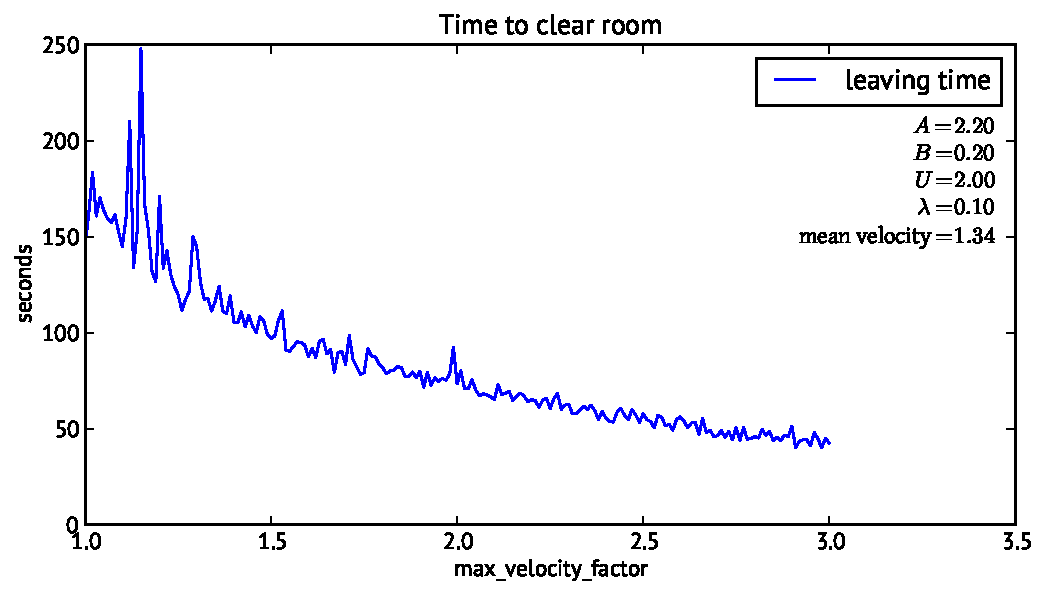
\includegraphics[scale=0.5]{Figures/fastIsSlowNot}
\caption{Fast is not slow}
\label{FastIsSlow}
\end{figure}
The larger the nervousness the faster is the evacuation. We have increased the max-velocity factor sow much that people eventually move through the walls. This start occurring around max-velocity-factor = 2.5, and measurements beyond this point are neglected.

Pedestrian flow rate is measure in the door opening, and the density of pedestrians in a 2 m by 2 m area directly in front of the door is measured. We also measure the time it takes for all pedestrians to leave the room.

The parameters for this simulation are the ones shown in \ref{Table_constants}

% TODO: Add parameters that are varied.


\subsection{The corridor scenario}
In this scenario we simulate pedestrians walking in both directions along a 20 
m long and six metres wide corridor. The pedestrians are divided into two 
groups, starting in opposite ends of the corridor and moving towards each 
other. The targets the pedestrians move towards are set 500 metres to each 
side, to make pedestrians walk in almost a straight line instead of converging 
towards the middle of the corridor. Flow rate is measured in the middle of the 
corridor, as is density. We start out with 100 pedestrians, adding a 
continuous inflow of three pedestrians per second, to simulate people arriving 
from outside the simulated area. Both the initial placement and the inflow of 
pedestrians are distributed randomly (i.e. approximately evenly) between the 
two ends of the corridor.

We expect to see lane formations through out our simulations
and the freezing by heating effect when we start raising the mean velocity
of the agents.

\subsubsection{Intial conditions and relaxation time $1,0$ second}

The parameters for this simulation are as in \ref{Table_constants} with the exception of the pedestrians
\begin{itemize*}
    \item Number of pedestrians: $50$ starting, adding $3/s$.
\end{itemize*}

When running the simulation we observe lane formations, and they almost clog up
in the corridor.

When we do a simulation with the max velocity factor set to $4.0$, instead of the normal $1.3$, the clogging
that occurs in the beginning eases up, and the pedestrians relatively fast
get out of the clogging and continuous toward their target. In this simulation
we also observe lane formations.

\begin{figure}[h]
\centering
\subfloat[The figure show the density in corridor when the parameters are set as \cite{ABconstant} and \cite{self-org}.]{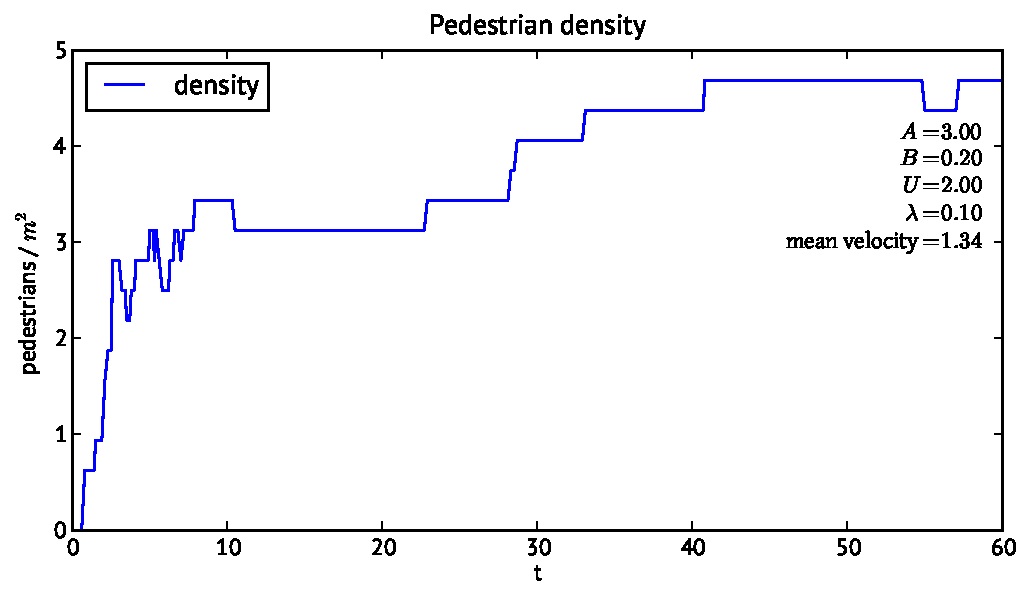
\includegraphics[scale=0.45]{Figures/dens_init_relax1.pdf}}
\subfloat[This figure shows the density in the corridor when the max velocity factor is set to $4.0$, and the other parameters as figure a.]{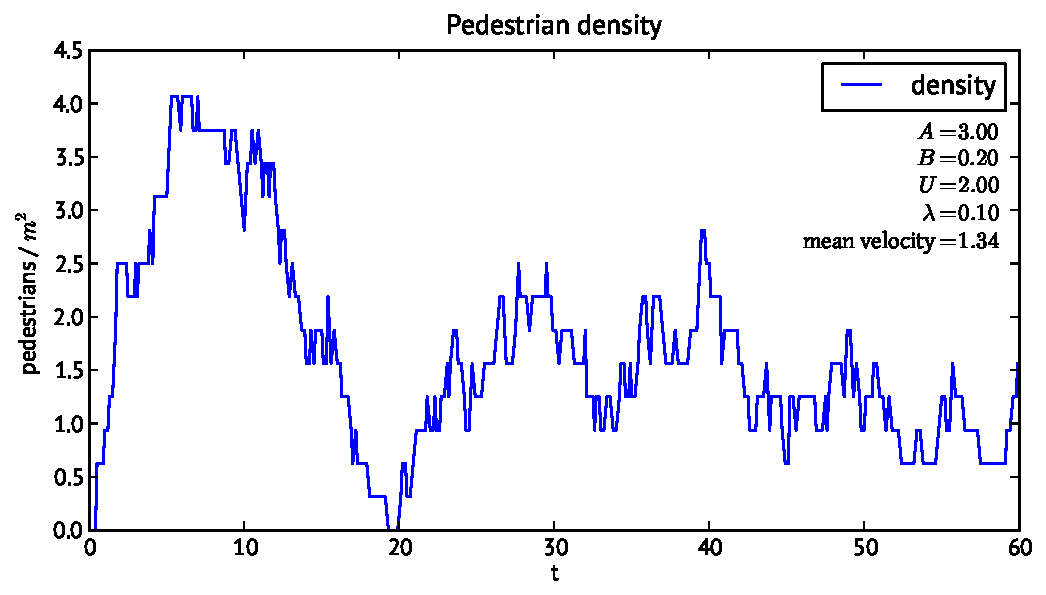
\includegraphics[scale=0.45]{Figures/dens_mvel4_relax1.pdf}}
\caption{These figures was made to see if the freezing by heating effect when raising the max velocity factor. As seen in the figures, the
density does not increase when the max desired velocity is increased. When raising the max desired velocity the density gets lower because
the pedestrians more easely get through the crowd.}
\label{fig:freezingbyheating1}
\end{figure}

\subsubsection{Intial conditions and relaxation time $0,5$ second}
\cite{helbing00} set the relaxation time to $0,5$. As the first corridor simulations we set the parameters as \cite{ABconstant}
and then change the relaxation time to $0,5$ as \cite{helbing00}. After the simulation with the initial conditions, we raise the
max desired velocity to see if we can replicate the freezing by heating effect.

The initial simulation has the values from \ref{Table_constants} with the exceptions:

\begin{itemize*}
    \item Relaxation time: $0,5 s$.
    \item Number of pedestrians: $50$ starting, adding $3/s$.
\end{itemize*}

The next simulation we keep the new relaxation time, but changes the max velocity factor set to $4.0$


When comparing the simulations we do not see the freezing by heating effect.
Instead we see that the pedestrians more easely escape the clogging, and the flow in each directions
gets more steady. In both simulations we observed lane formation.

\begin{figure}[h]
\centering
\subfloat[The figure show the density in corridor when the parameters are set as \cite{ABconstant} and \cite{helbing00}.]{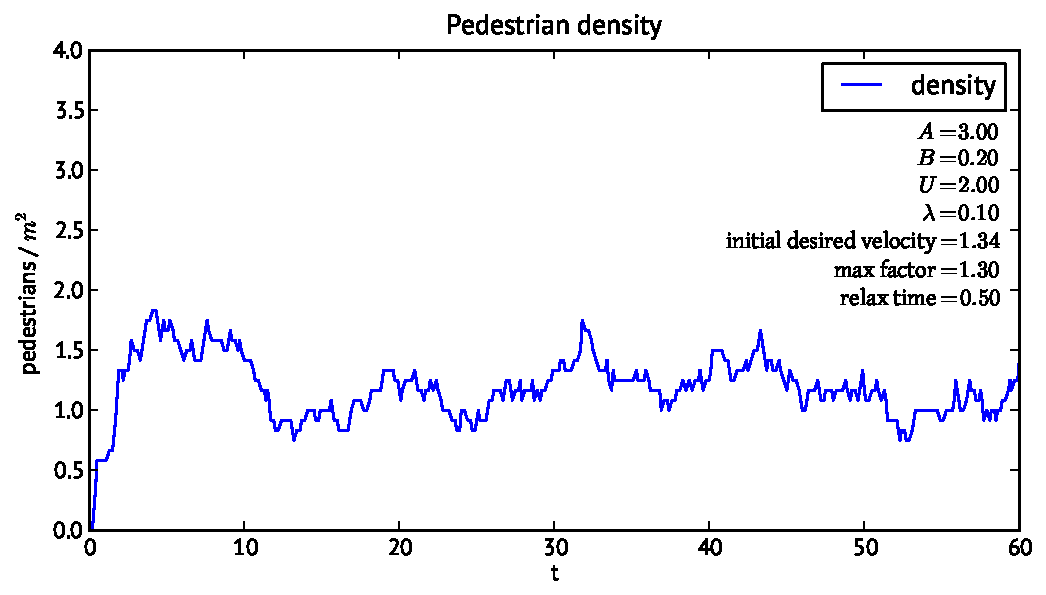
\includegraphics[scale=0.45]{Figures/dens_init_relax05.pdf}}
\subfloat[This figure shows the density in the corridor when the max velocity factor is set to $4.0$ and the max desired velocity is set to $4,0$, and the other parameters as figure a.]{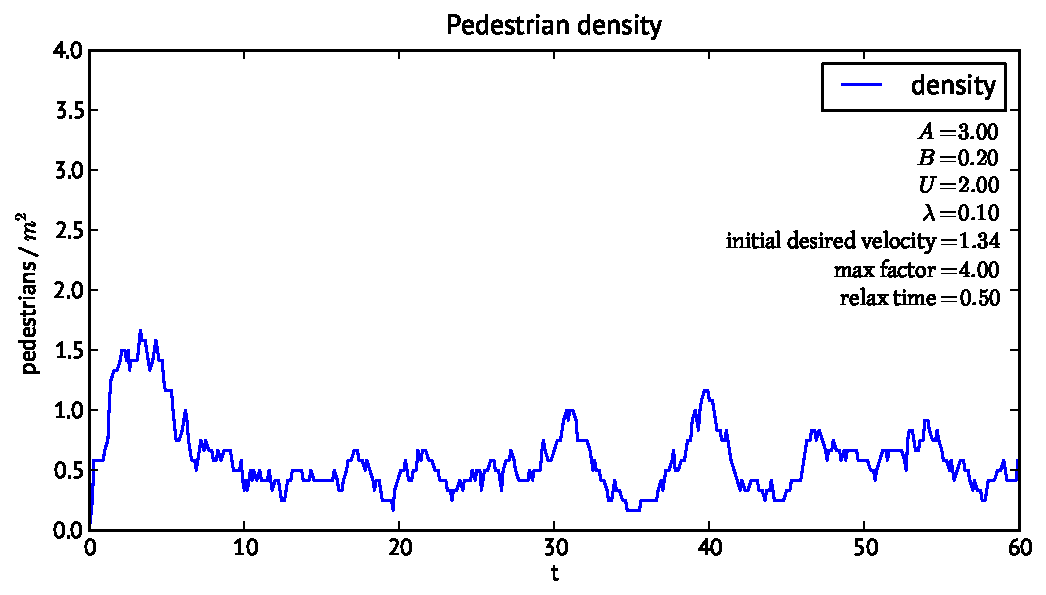
\includegraphics[scale=0.45]{Figures/dens_mvel4_relax05.pdf}}
\caption{These figures was made to see if the freezing by heating effect when raising the max velocity factor. As seen in the figures, the
density does not increase when the max desired velocity is increased. When raising the max desired velocity the density gets lower because
the pedestrians more easely get through the crowd. The difference between figure \ref{fig:freezingbyheating1} and this is the relation time,
respectively $1,0$ and $0,5$.}
\label{fig:freezingbyheating05}
\end{figure}

\subsection{The bottleneck}
In this scenario we wanted to the the oscillitory flows that is reported 
in \cite{self-org} to happen when you have a bidirectional flaw through a 
bottleneck. A print screen from the simulation is shown in figure 
\ref{fig:bottleneckbidirec}.

\begin{figure}[h]
\centering
{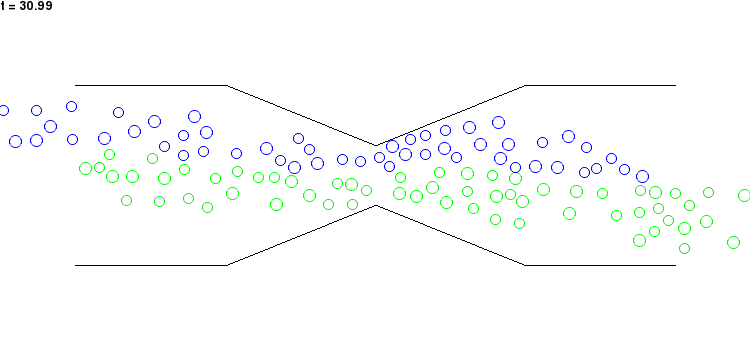
\includegraphics[scale=0.35]{Figures/bottleneck.png}}
\caption{A screen shot of the bottleneck simulation.}
\label{fig:bottleneckbidirec}
\end{figure}

\subsubsection{Attempts to see the faster is slower effect in the bottleneck}
In order to see the faster-is-slower effect we make a series of simulations 
with increasing mean velocity. The results is presented in figure 
\ref{fig:is-faster-slower-in-bottleneck}.

\begin{figure}[h]
\centering
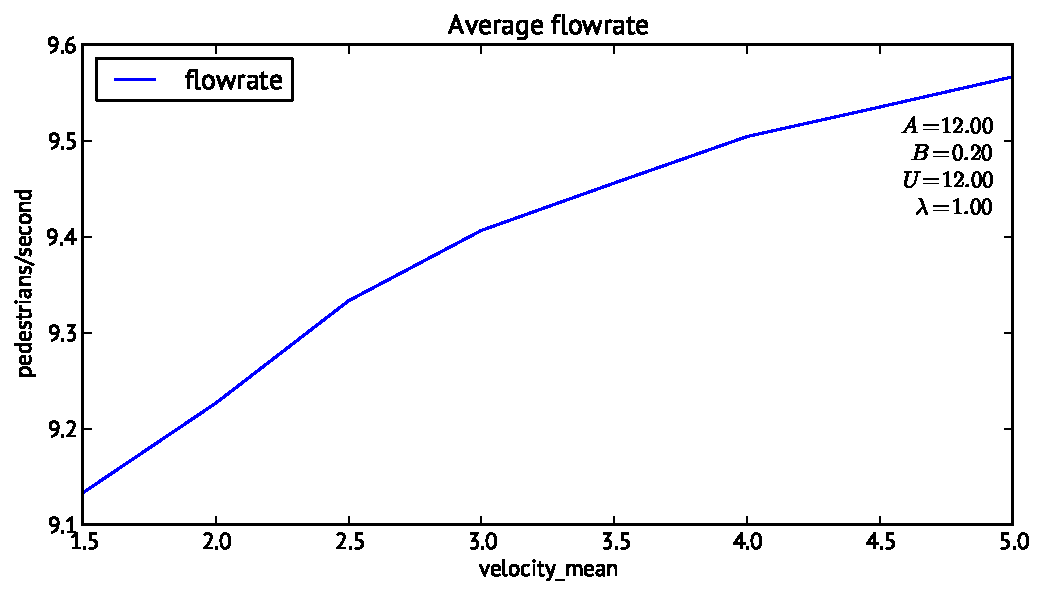
\includegraphics[scale=0.45]{Figures/Wide-kink-one-directional-flowrate-agg.pdf}
\caption{A graph of the flow rate as the average velocity is increased}
\label{fig:is-faster-slower-in-bottleneck}
\end{figure}

\subsection{The corridor with open space}
In this scenario we wanted to reproduce the results that people start to 
clock up in a corridor if there is a sudden area that allow pedestrians to try 
and overtake each other. To see if the flow rate is affected by the pedestrians 
who try to overtake each other we compare the flow rate with the wide space with 
the flow rate from a normal corridor scenario. A screen shot from each simulation 
can be seen in figure \ref{fig:widekink}.

\begin{figure}[h]
\centering
\subfloat[A screen shot of the normal corridor.]{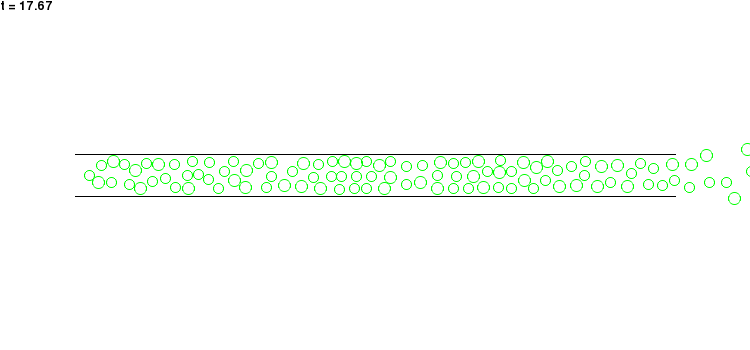
\includegraphics[scale=0.25]{Figures/normalcorridor.png}}
\subfloat[A screen shot of the corridor with a wide space.]{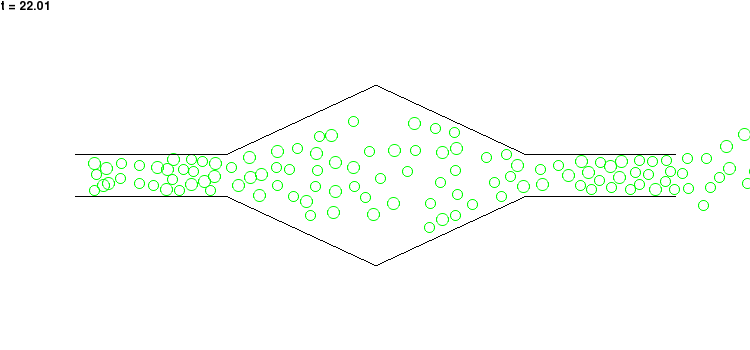
\includegraphics[scale=0.25]{Figures/Widespace.png}}
\caption{The two scenarios we want to compare to see the effect of the wide space.}
\label{fig:chokepoint}
\end{figure}

We expected to see that the flow rate in the scenario shown in figure 
\ref{fig:chokepoint} (b) would be lower than in the scenario (a). What we sat 
in shown in figure \ref{fig:effect-of-widespace}

\begin{figure}[h]
\centering
\subfloat[A graph of the mean velocity of the pedestrians in normal corridor]{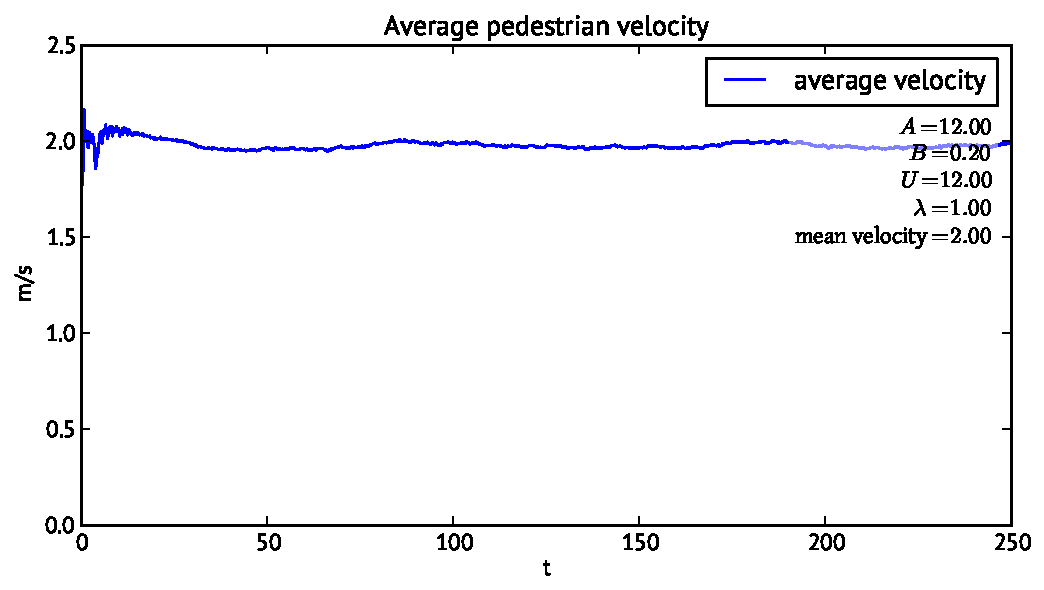
\includegraphics[scale=0.45]{Figures/corridor-velocity.pdf}}
\subfloat[A graph of the mean velocity of the pedestrian in the corridor with a wide space]{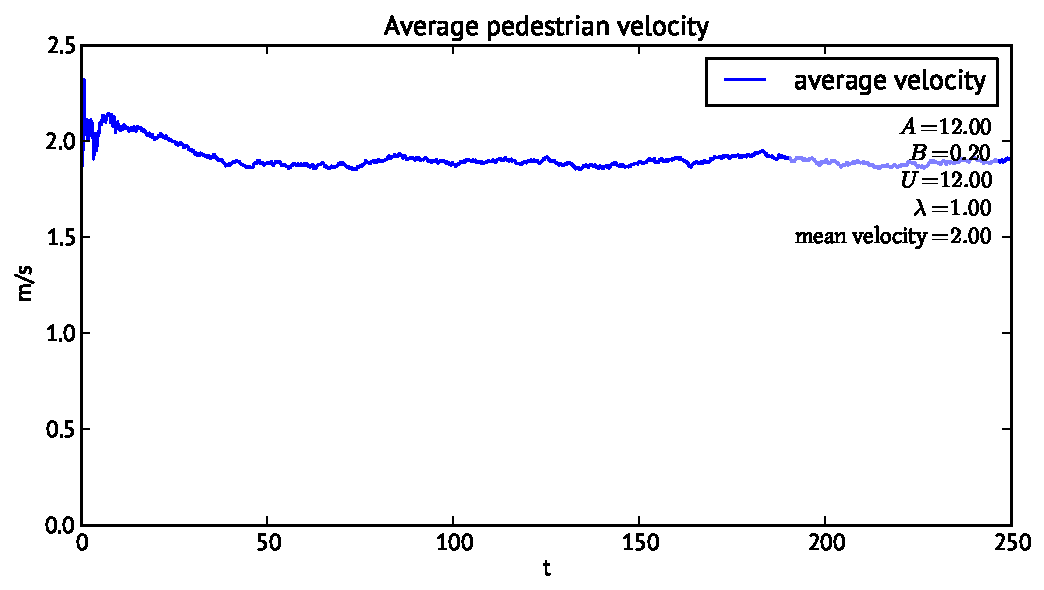
\includegraphics[scale=0.45]{Figures/bottleneck-velocity.pdf}}\\
\subfloat[A graph of the flow rate of the pedestrians in the normal corridor]{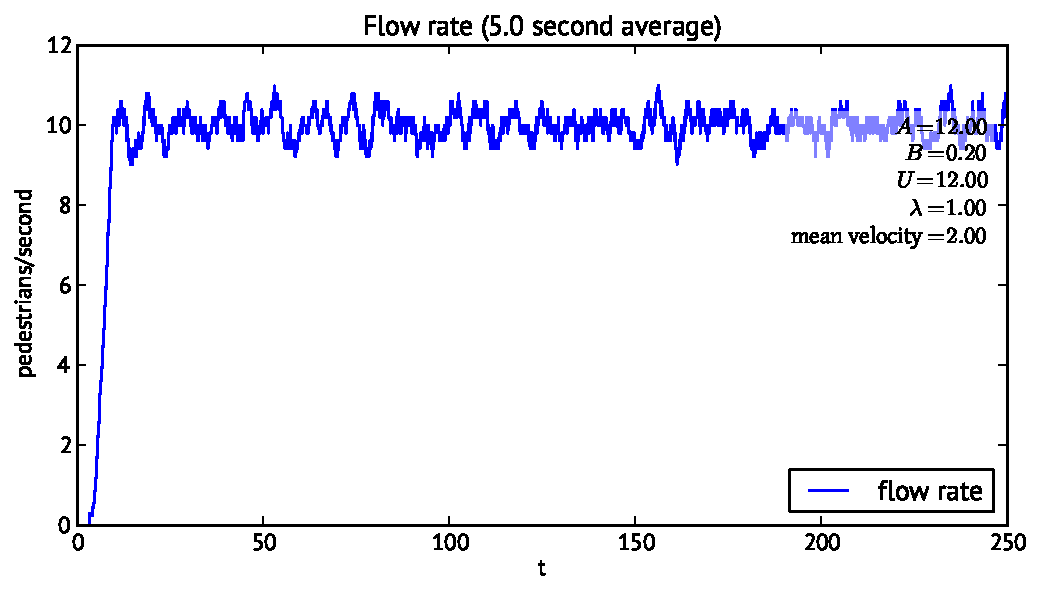
\includegraphics[scale=0.45]{Figures/corridor-flowrate.pdf}}
\subfloat[A graph of the flowrate in the corridor with the wide space]{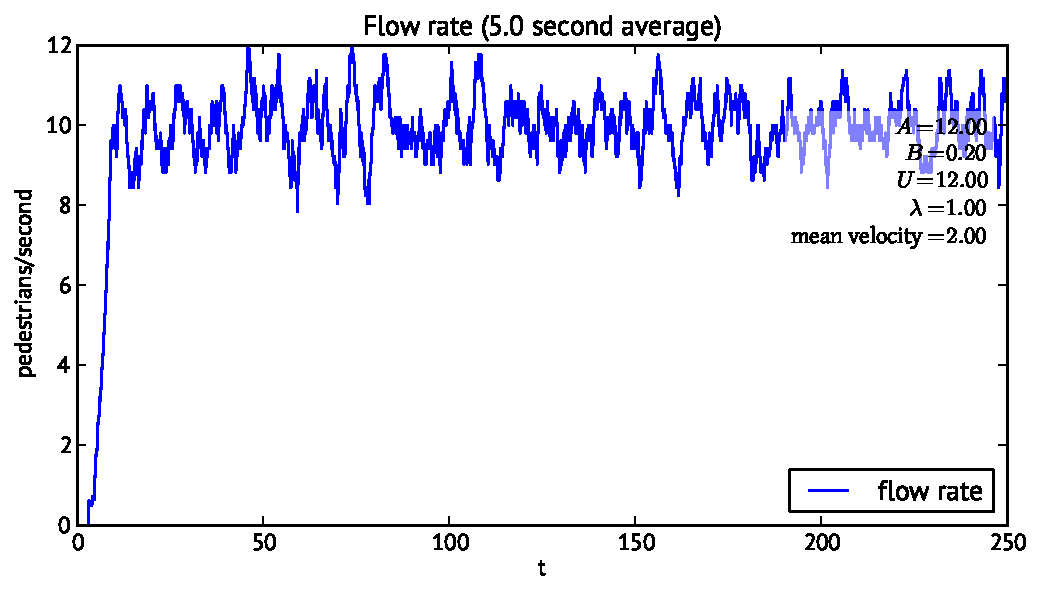
\includegraphics[scale=0.45]{Figures/bottleneck-flowrate.pdf}}
\caption{There is a lowering of the average velocity of the pedestrians due to the bottleneck. We see that there is no consistent lowering of the flowrate due to the bottleneck. What we see is that the flowrate is varying more over time.}
\label{fig:effect-of-widespace}
\end{figure}

\subsubsection{Attempts to see the faster is slower effect in the corridor with wide space}
The faster is slower effect in not observed in the extent that we would expect from 
the article. However the flow rate does not increase linearly with average velocity. 
 
\begin{figure}[h]
\centering
\subfloat[A graph of the flow rate as the average velocity is increased in the case of one directional pedestrian flow.]{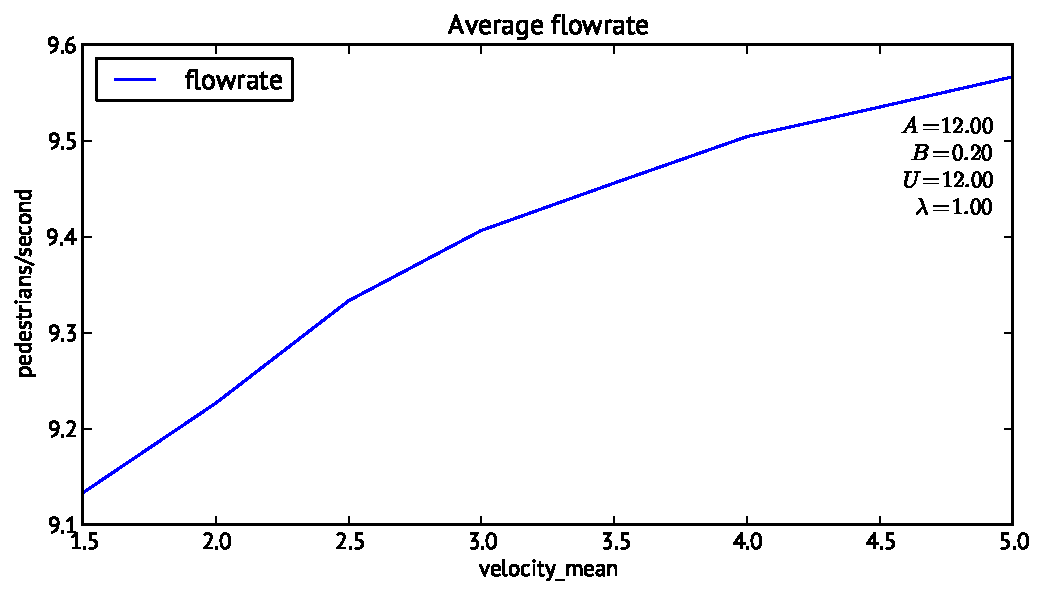
\includegraphics[scale=0.45]{Figures/Wide-kink-one-directional-flowrate-agg.pdf}}
\subfloat[A graph of the flow rate as the average velocity is increased in the case of bidirectional pedestrian flow.]{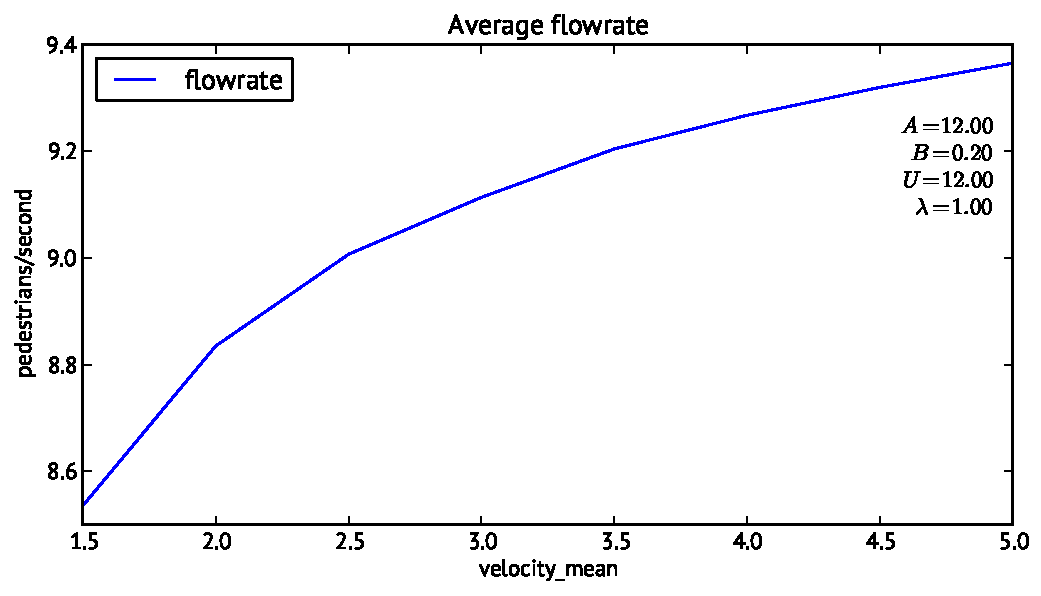
\includegraphics[scale=0.45]{Figures/Widekink-twodirectional-flowrate-agg.pdf}}
\caption{The two scenarios we want to compare to see the effect of the wide space.}
\label{fig:is-faster-slower-in-widekink}
\end{figure}

% TODO: Add parameters that are varied.

\clearpage
% vim:ft=tex
\section{Conclusion}
\label{sec:conclusion}

\subsection{Further work}
Since the simulation we present in the report has not shown some properties of 
a crowd, if given more time our group would like try to solve the 
discrepancies and add the possible solutions that has been talked about in 
section \ref{sec:discussion}. The first thing to do maybe modify the repulsive 
forces and add the frictional force, and make them velocity dependent, which 
will make the crowd behave more realistic.  To enable the model to simulate 
more complex situation, we will need the path finding feature. Also a set of 
parameters should be determined when the environment is changed, and the 
method to attain those parameters may be the same as what the Helbing group 
has been doing, that is by doing some experiments and analysing the video 
track.

\clearpage
\section{Perspectives}
\label{sec:perspectives}

\clearpage
% vim:ft=tex
\section{Appendix}
\section{calculation}
In this simplified situation, there is no wall and only one other pedestrian $\beta$ at position $(-\frac{\sqrt{2}}{5}, \frac{\sqrt{2}}{5})$ which exert expelling force to $\alpha$.  The exit is reduced to one point $E(4,4)$.  Their positions at $t=0$ is shown in the drawing below:\\

\begin{figure}
\centering
{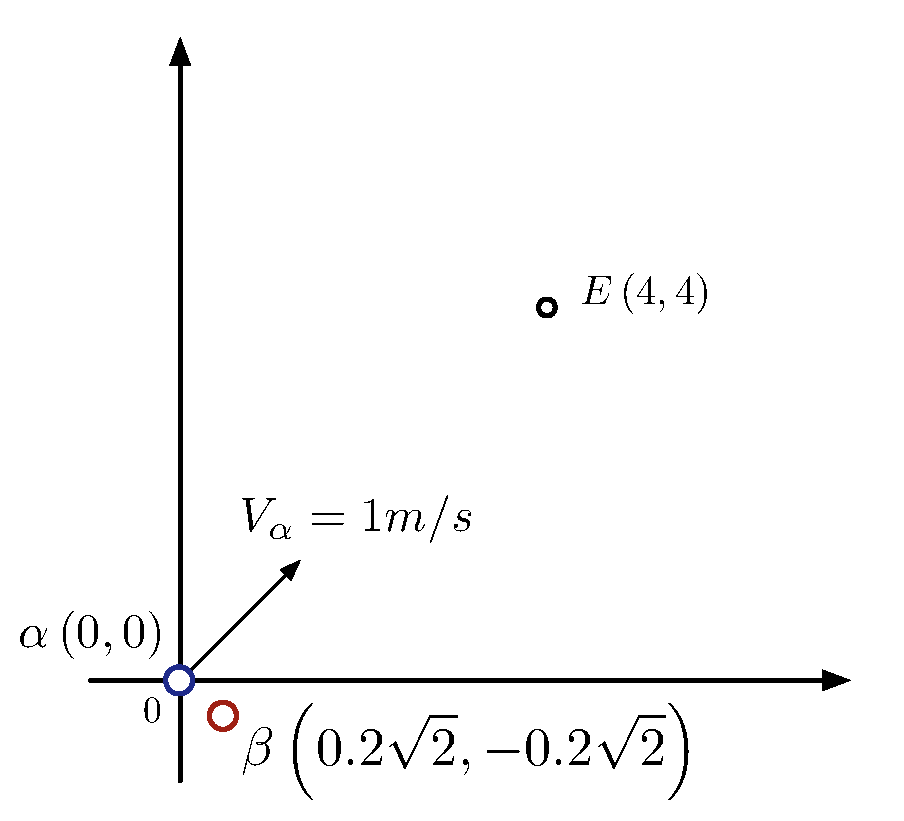
\includegraphics[scale=0.45]{calculation.pdf}} 
\caption{\small{}\label{calc}}
\end{figure}

In addition, to complete the initial conditions, we need to know $\alpha$'s actual velocity at $t=0$, suppose $\overrightarrow{v_{\alpha}(0)}=(\frac{\sqrt{2}}{2}, \frac{\sqrt{2}}{2})$, also the average speed into the desired direction of motion $\overline{v_{\alpha}(0)}=0$.\\

With those numbers we can calculate the impatience factor 
 \begin{equation}
 n_{\alpha}(0)=1-\frac{\overline{v_{\alpha}(0)}}{v^{0}_{\alpha}(0)}=1-\dfrac{0}{v^{0}_{\alpha}(0)}=1
 \end{equation}

so 
 \begin{equation}
 v^{0}_{\alpha}(0)=[1-n_{\alpha}(0)]v^{0}_{\alpha}(0) + n_{\alpha}(0)v_{\alpha}^{max} = v_{\alpha}^{max}
 \end{equation}
 
Suppose $v_{\alpha}^{max}=3$, then 

 \begin{equation}
 	\vec{f^{0}_{\alpha}} \left( \vec{v_{\alpha}} \right) 
= 	\frac{1}{\tau_{\alpha}} \left( v^{0}_{\alpha} 
	\vec{e_{\alpha}} - \vec{v_{\alpha}} \right)
 \end{equation}
 
where $\tau_{\alpha}=1$,
 \begin{equation}
 \overrightarrow{f^{0}_{\alpha}}\overrightarrow{v_{\alpha}} = (\sqrt{2}, \sqrt{2})
 \end{equation}

Another part of $\alpha$'s acceleration is from the repelling force from $\beta$, in order to speed  up the calculation here we omit the not so important part in calculating $\overrightarrow{f_{\alpha \beta}}$.
Therefore,
 \begin{equation}
 \overrightarrow{f_{\alpha \beta}} = A^{2}_{\alpha} exp(\frac{r_{\alpha\beta}-d_{\alpha\beta}}{B^{2}_{\alpha}})\overrightarrow{n_{\alpha \beta}}
 \end{equation}
where $A^{2}_{\alpha}=3, B^{2}_{\alpha}=0.2, r_{\alpha\beta}=0.6, d_{\alpha\beta}=0.4$, and $\overrightarrow{n_{\alpha \beta}}=(-\frac{\sqrt{2}}{2}, \frac{\sqrt{2}}{2})$,
so 
 \begin{equation}
 \overrightarrow{f_{\alpha \beta}} = 8(-\frac{\sqrt{2}}{2}, \frac{\sqrt{2}}{2})
 \end{equation}
In all, the acceleration of $\alpha$ is 
 \begin{equation}
 \overrightarrow{f_{\alpha}(0)} = \overrightarrow{f^{0}_{\alpha}}\overrightarrow{v_{\alpha}} + \overrightarrow{f_{\alpha\beta}} = (-3\sqrt{2}, 5\sqrt{2})
 \end{equation}
Now we are ready to calculate where $\alpha$ is after $\bigtriangleup t=0.1$, if we assume $\alpha$ moves with a constant acceleration during that small time interval.
As the motion is in two dimensions, we need to calculate the displacement in $x$ and $y$ axis respectively.

 \begin{equation}
 r^{x}_{\alpha} = v^{x}_{\alpha} \bigtriangleup t + \frac{1}{2} f^{x}_{\alpha} \bigtriangleup t ^{2}
 \end{equation}
 
 For the y direction,
  \begin{equation}
 r^{y}_{\alpha} = v^{y}_{\alpha} \bigtriangleup t + \frac{1}{2} f^{y}_{\alpha} \bigtriangleup t ^{2}
 \end{equation}
 Therefore, $r_{\alpha}(0.1)= (0.05, 0.1)$
\subsection{Table of notation}
\begin{center}
\begin{tabular}{lll}
\hline
\multicolumn{3}{|c|}{\emph{List of constants and variables}}\\
\hline
\small{\textbf{Symbol}} & \small{\textbf{Description}} & \small{\textbf{Unit}}\\
\hline
$A_{\alpha}^{1}$ & \small{Controls the strength of the personal space force}\\
\hline
$A_{\alpha}^{2}$ & \small{Controls the strength of physical collisions}  & \\
\hline
$B_{\alpha}^{1}$ & \small{Controls the range of the personal space force} & \\
\hline
$B_{\alpha}^{2}$ & \small{Controls the range of physical collisions} & \\
\hline
$\lambda_{\alpha}$ & The anisotropic character of pedestrian interaction & \\
\hline
$\vec{f_{\alpha}} \left( t \right)$ & All forces acting on pedestrian $\alpha$  & \\
\hline
$\vec{f_{\alpha B}} \left( \vec{r_{\alpha}} \right)$ & Force on pedestrian $\alpha$ from walls & \\
\hline
$\vec{f_{\alpha \beta}} \left( \vec{r_{\alpha}}, \vec{r_{\beta}}, \vec{V_{\alpha}}, \vec{V_{\beta}} \right)$ & Force on pedestrian $\alpha$ from pedestrian $\beta$ & \\
\hline
$\vec{f_{\alpha i}} \left( \vec{r_{\alpha}}, \vec{r_{i}}, t \right)$ & Force on pedestrian $\alpha$ from attractions & \\
\hline
$V_{\alpha}^{0}$ & Initial speed of pedestrian $\alpha$ & \\
\hline
$V_{\alpha}^{\text{max}}$ & Maximum speed of pedestrian $\alpha$ & \\
\hline
$\vec{V_{\alpha}^{\text{0}}}$ & Desired velocity of pedestrian $\alpha$ & \\
\hline
$\overline{V}_{\alpha}$ & Average speed in desired direction & \\
\hline
$\vec{e}_{\alpha}$ & Vector pointing in desired direction of pedestrian $\alpha$ & \\
\hline
$\vec{r}_{\alpha}\left( t \right) $ & Vector pointing to position of pedestrian $\alpha$ at time t & \\
\hline
$\vec{r}_{B}$ & Vector pointing to nearest point of wall & \\
\hline
$r_{\alpha}$ & Radius of pedestrian $\alpha$ & \\
\hline
$r_{\beta}$ & Radius of pedestrian $\beta$ & \\
\hline
$r_{\alpha \beta}$ & The sum of the radii of pedestrian $\alpha$ and $\beta$ & \\
\hline
$\vec{X}_{\alpha}$ & Vector pointing to center of mass of pedestrian $\alpha$ & \\
\hline
$\vec{X}_{\beta}$ & Vector pointing to center of mass of pedestrian $\beta$ & \\
\hline
$d_{\alpha \beta}$ & Distance between center of mass of pedestrian $\alpha$ and $\beta$ & \\
\hline
$\tau_{\alpha}$ & Relaxation time $\alpha$ and $\beta$ & \\
\hline
$\eta_{\alpha}$ & Impatience of pedestrian $\alpha$ at time t & \\
\hline
$\vec{\eta}_{\alpha \beta}\left( t \right)$ & Normal vector pointing from $\alpha$ to $\beta$ at time t & \\
\hline
$\vec{\xi}\left( t \right)$ & Stochastic element & \\
\hline
$\phi_{\alpha \beta} \left( t \right)$ & Angle between pedestrian $\alpha$ and $\beta$ & \\
\hline
\label{tableofconstandvar}
\end{tabular}
\end{center}
\clearpage
\bibliographystyle{ruc}
\bibliography{crowd-modelling}
\clearpage

\end{document}